\documentclass[oneside,11pt]{memoir}

\usepackage{amsmath}
\usepackage{graphicx}

\usepackage[usenames,dvipsnames]{color}
\usepackage[pdftex, pdfstartview = {FitH}]{hyperref}

\usepackage{anyfontsize}

\usepackage{makeidx}

\usepackage{placeins}

% to use minted
%   install the pygments package for python
%   sudo apt-get install python-pygments
%   get the style file, minted.sty
%     http://code.google.com/p/minted/downloads/detail?name=minted.sty
%   resources
%     http://stackoverflow.com/questions/1966425/source-code-highlighting-in-latex#1985330
%     http://mirror.unl.edu/ctan/macros/latex/contrib/minted/minted.pdf
%     also see minted.pdf in practical documentation
%   running pdflatex:
%     pdflatex -shell-escape nexus_user_guide.tex
\usepackage{minted}


\hypersetup{
    colorlinks=true,
    citecolor = Blue,
    linkcolor = Blue,
    urlcolor  = Blue,
    pdfborder={0 0 0},
}


\makeindex

%\chapterstyle{hangnum}
\chapterstyle{verville}


\numberwithin{equation}{section}

\setlength{\hoffset}{0in}
\setlength{\voffset}{-0.5in}
\setlength{\marginparwidth}{1.0in}
\setlength{\oddsidemargin}{1.0in}
\setlength{\evensidemargin}{1.0in}
\addtolength{\textwidth}{1.0in}
\addtolength{\textheight}{1.0in}
\setlength{\spinemargin}{1.25in}
\setlength{\foremargin}{1.25in}
\addtolength{\textwidth}{-8pt}
\checkandfixthelayout


\newcommand{\hide}[1]{}
%\newcommand{\hide}[1]{{#1}}

%\newcommand{\condense}[1]{This content has been temporarily redacted to produce a shorter document.}
\newcommand{\condense}[1]{{#1}}


  \newcommand{\abs}[1]{\lvert #1 \rvert}
  \newcommand{\norm}[1]{\lVert #1 \rVert}
  \newcommand{\pnorm}[2]{\lVert #1 \rVert_{#2}}
  \newcommand{\mean}[1]{\langle #1 \rangle}

  \newcommand{\ket}[1]{\lvert #1 \rangle}
  \newcommand{\bra}[1]{\langle #1 \rvert}
  \newcommand{\expval}[3]{\bra{#1}\hat{#2}\ket{#3}}
  \newcommand{\expvalnh}[3]{\bra{#1}#2\ket{#3}}
  \newcommand{\overlap}[2]{\langle #1 \lvert #2 \rangle}


  \newcommand{\sstitle}[1]{\textbf{\underline{#1}}\newline}
  \newcommand{\bu}[1]{\textbf{\underline{#1}}}

  \newcommand{\HRule}{\rule{\linewidth}{0.5mm}}



\frontmatter


\newenvironment{changemargin}[2]{%
\begin{list}{}{%
%\setlength{\topsep}{0pt}%
\setlength{\leftmargin}{#1}%
\setlength{\rightmargin}{#2}%
%\setlength{\listparindent}{\parindent}%
%\setlength{\itemindent}{\parindent}%
%\setlength{\parsep}{\parskip}%
}%
\item[]}{\end{list}}




\begin{document}

\definecolor{shadecolor}{gray}{0.9}


\thispagestyle{empty}
\begin{changemargin}{-1cm}{-1cm}
  \begin{center}
    \hspace{1cm}\\
    \hspace{1cm}\\
    \hspace{1cm}\\
    \hspace{1cm}\\
    \hspace{1cm}\\
    \hspace{1cm}\\
    \hspace{1cm}\\
    \hspace{1cm}\\
    \hspace{1cm}\\
    \hspace{1cm}\\
    \hspace{1cm}\\
    \hspace{1cm}\\
    \HRule\\
    \vspace{4mm}
    \textbf{\fontsize{40}{45}\selectfont The Nexus User Guide} \\ 
    \HRule\\
    \vspace{1cm}
    \vspace{6cm}
    Version 1.6.0 \\
    \vspace{1 cm}
    By Jaron T. Krogel \\
    \vspace{1cm}
    \today
  \end{center}
\end{changemargin}
\pagebreak

\tableofcontents



\mainmatter

\pagebreak
\chapter{Using this document} \label{usedoc}

The Nexus User Guide provides an overview of Nexus (Sec. Sec. \ref{sec:overview}), instructions on how to install it (Sec. \ref{sec:installation}), an explanation of Nexus user scripts used to create simulation workflows (Sec. \ref{sec:user_scripts}), and complete examples of electronic structure calculations using Nexus (Sec. \ref{sec:examples}).  Reading all sections is recommended prior to beginning production work.  The impatient may quickly visit ``Nexus Installation'' (Sec. \ref{sec:installation}) and see the examples section (Sec. \ref{sec:examples}) for template calculations to begin using Nexus immediately. If you cannot find what you need in this document, contact the main developer of Nexus (Jaron Krogel), at krogeljt@ornl.gov (but please make a thorough search first!).

Some basic understanding of Python is recommended for Nexus users.  For a very quick introduction to the basics, read Appendix \ref{app:python_basics}.  More information can be found under ``Brushing up on Python'' in the ``Recommended Reading'' Section (Sec. \ref{sec:learn_python}).

This document also provides a brief overview of Quantum Monte Carlo (QMC) from an applied perspective (Appendix \ref{app:theory}) and directions on where to go to learn more (Sec. \ref{sec:reading}).  Consider reading ``QMC Practice in a Nutshell'' (Appendix \ref{app:theory}) and the review articles and online resources listed under ``Quantum Monte Carlo: Theory and Practice'' (Sec. \ref{sec:learn_qmc}) before proceeding to the overview (Sec. \ref{sec:overview}) and the examples (Sec. \ref{sec:examples}).  

%For fine-grained information about Nexus's many features, consult the ``Nexus User Reference'' (\ref{sec:reference}).



\pagebreak
\chapter{Overview of Nexus} \label{sec:overview}
\section{What Nexus is}
Nexus is a collection of tools, written in Python, to perform 
complex electronic structure calculations and analyze the results.  The main 
focus is currently on performing arbitrary Quantum Monte Carlo (QMC) 
calculations with QMCPACK, however VASP, Quantum Espresso, and GAMESS are
also supported.  A single QMC calculation typically requires several 
previous calculations with other codes to produce a starting guess for the 
many-body wavefunction and convert it into a form that QMCPACK understands.  
Managing the resulting array of calculations, and the flow of information 
between them, quickly becomes unweildy to the researcher, demands a great 
deal of human time, and increases the potential for human error.  Nexus 
reduces both the human time required and potential for error by 
automating the total simulation process.  

\section{What Nexus can do}
The capabilities of Nexus currently include crystal structure 
generation, standalone Density Functional Theory (DFT) calculations with 
PWSCF (Quantum Espresso) or VASP,  quantum chemical calculations with GAMESS,  
Hartree-Fock (HF) calculations of atoms with the SQD code (packaged with 
QMCPACK), complete QMC calculations with QMCPACK (including wavefunction 
optimization, Variational Monte Carlo (VMC), and Diffusion Monte Carlo (DMC) in 
periodic or open boundary conditions), automated job management on workstations 
(by acting as a virtual queue) and clusters/supercomputers  
including handling of dependencies 
between calculations and job bundling,  and extraction of results from 
completed calculations for analysis.  The integration of these capabilities 
permits the user to focus on the high-level tasks of problem formulation and 
interpretation of the results without (in principle) becoming too involved 
in the time-consuming, lower level details.

\section{How Nexus is used}
Use of Nexus currently involves writing a short Python script 
describing the calculations to be performed.  This small script formed by the 
user closely resembles an input file for electronic structure codes.  A key 
difference is that this ``input file'' represents executable code, and so 
variables are easily defined for use in expressions and more complicated 
simulation workflows (\emph{e.g.} an equation of state) can be constructed 
with if/else logic and for loops.  Knowledge of the Python programming language 
is helpful to perform complex calculations, but not essential for use of  
Nexus.  Starting from working ``input files'' such as those covered 
in the ``Complete Examples'' section (\ref{sec:examples}) is a good way to proceed. 




\pagebreak
\chapter{Nexus Installation} \label{sec:installation}
Installation of Nexus can be accomplished by 
%a single download from \texttt{qmcpack.org} and 
setting a single environment variable provided a 
working python environment exists. 


%\section{Downloading Nexus}
%To download Nexus, go to \url{http://qmcpack.org/downloads/} and 
%select the latest release of QMCPACK.  Save the \texttt{tar.gz} file 
%to your hard drive and unpack it (\texttt{tar -xzf qmcpack*.tgz}.  
%Nexus can be found in \texttt{./qmcpack/nexus/}.  Throughout this document, 
%the path leading up to the \texttt{nexus} directory is referred to as \texttt{/your\_download\_path}.


\section{Setting environment variables}
To make your Python installation (must be Python 2.x as 3.x is not supported) 
aware of Nexus, simply set the PYTHONPATH environment variable.  For example, in bash this would look like:
\begin{shaded}
\begin{verbatim}
export PYTHONPATH=/your_download_path/nexus/lib:$PYTHONPATH
\end{verbatim}
\end{shaded}
\noindent
Add this to \emph{e.g.} your .bashrc file to make Nexus available 
in future sessions.
If you want to use the command line tools, add them to your path:
\begin{shaded}
\begin{verbatim}
export PATH=/your_download_path/nexus/bin:$PATH
\end{verbatim}
\end{shaded}
%Add these to \emph{e.g.} your .bashrc file to make Nexus available 
%to future sessions.

Both of these environment variables can be set automatically by the \texttt{install} script packaged with Nexus.  To use the installer, instead of performing the manual installation above, simply type the following at the command line:
\begin{shaded}
\begin{verbatim}
/your_download_path/nexus/install
\end{verbatim}
\end{shaded}
\noindent
If you want the Nexus binaries to reside a location different than \texttt{/your\_download\_path/nexus/bin}, simply provide this path to the installer:
\begin{shaded}
\begin{verbatim}
/your_download_path/nexus/install /some/other/location
\end{verbatim}
\end{shaded}

\section{Installing Python dependencies}
In addition to the standard Python installation, the \texttt{numpy} module must 
be installed for Nexus to function at a basic level.  To realize 
the full range of functionality available, it is recommended that the 
\texttt{scipy}, \texttt{matplotlib}, and \texttt{h5py} modules be installed as 
well.  Many of these packages are already available in various supercomputing 
environments.  On a debian-based Linux system, such as Ubuntu, installation of 
these python modules is easily accomplished by invoking the following at the 
command line:
\begin{shaded}
\begin{verbatim}
sudo apt-get install python-numpy
sudo apt-get install python-scipy python-matplotlib python-h5py 
\end{verbatim}
\end{shaded}
\noindent
To install the Python modules on other platforms, please see 
``Helpful Links for Installing Python Modules'' (section \ref{sec:install_python}).

Of course, to run full calculations, the simulation codes and converters 
involved must be installed as well.  These include a modified version of 
Quantum Espresso (\texttt{pw.x}, \texttt{pw2qmcpack.x}, optionally 
\texttt{pw2casino.x}), QMCPACK (\texttt{qmcpack}, \texttt{qmcpack\_complex}, \texttt{convert4qmc}, \texttt{wfconvert}, \texttt{ppconvert}), 
SQD (\texttt{sqd}, packaged with QMCPACK), VASP, and/or GAMESS.  
Complete coverage of this task is beyond the scope of the current document, but 
please see ``Helpful Links for Installing Electronic Structure Codes'' 
(section \ref{sec:install_code}).






\pagebreak
\chapter{Nexus User Scripts} \label{sec:user_scripts}

Users interact with Nexus by writing a Python script that often resembles an input file.  A Nexus user script typically consists of six main sections, as described below:

\begin{description}
  \item[Nexus imports:] functions unique to Nexus are drawn into the user environment.
  \item[Nexus settings:] specify machine information and configure the runtime behavior of Nexus.
  \item[Physical system specification:]  create a data description of the physical system.  Generate a crystal structure or import one from an external data file.  Physical system details can be shared among many simulations.
  \item[Workflow specification:] describe the simulations to be performed.  Link simulations together by their data dependencies to form workflows.
  \item[Workflow execution:] pass control to Nexus for active workflow management.  Simulation input files are generated, jobs are submitted and monitored, output files are collected and preprocessed for later analysis.
  \item[Data analysis:] control returns to the user to extract preprocessed simulation output data for further analysis. 
\end{description}


Each of the six input sections is the subject of lengthier discussion: ``Nexus imports'' (Sec. \ref{sec:user_imports}), ``Nexus settings'' (\ref{sec:user_settings}), ``Physical system specification'' (\ref{sec:user_system}),  ``Workflow specification'' (\ref{sec:user_workflows}), ``Workflow execution'' (\ref{sec:user_execution}), ``Data analysis'' (\ref{sec:user_data_analysis}).  These sections are also illustrated in the abbreviated example script below.  For more complete examples and further discussion, please refer to the user walkthroughs in Sec. \ref{sec:examples}.



\section{Nexus imports}\label{sec:user_imports}
Each script begins with imports from the main Nexus module.  Items imported include the interface to provide settings to Nexus, helper functions to make objects representing atomic structures or simulations of particular types (\emph{e.g.} QMCPACK or VASP), and the interface to provide simulation workflows to Nexus for active management. 

The import of all Nexus components is accomplished with the brief ``\texttt{from nexus import *}''.  Each component can also be imported separately by name, as in the example below.
\begin{minted}{python}
from nexus import settings                   # Nexus settings function
from nexus import generate_physical_system   # for creating atomic structures
from nexus import generate_pwscf             # for creating PWSCF sim. objects
from nexus import Job                        # for creating job objects
from nexus import run_project                # for active workflow management
\end{minted}

\noindent
This has the advantage of avoided unwanted namespace collisions with user defined variables.
The major Nexus components available for import are listed in Table \ref{tab:imports}.

\FloatBarrier
\begin{table}[h]
\begin{center}
\begin{tabularx}{\textwidth}{l l}
   \hline
   \bfseries component                 & \bfseries description \\
   \hline
   \texttt{settings}                   & Alter runtime behavior.  Provide machine information.    \\
   \texttt{generate\_physical\_system} & Create atomic structure including electronic information.  \\
   \texttt{generate\_structure}        & Create atomic structure without electronic information.    \\
   \texttt{generate\_simulation}       & Create generic simulation object.    \\
   \texttt{generate\_pwscf}            & Create PWSCF simulation object.    \\
   \texttt{generate\_vasp}             & Create VASP simulation object.    \\
   \texttt{generate\_gamess}           & Create GAMESS simulation object.    \\
   \texttt{generate\_qmcpack}          & Create QMCPACK simulation object.    \\
   \texttt{generate\_sqd}              & Create SQD simulation object.    \\
   \texttt{input\_template}            & Create generic input file object. \\
   \texttt{multi\_input\_template}     & Create generic input file object representing multiple files.\\
   \texttt{generate\_pwscf\_input}     & Create PWSCF input file object.    \\
   \texttt{generate\_vasp\_input}      & Create VASP input file object.    \\
   \texttt{generate\_gamess\_input}    & Create GAMESS input file object.    \\
   \texttt{generate\_qmcpack\_input}   & Create QMCPACK input file object.    \\
   \texttt{generate\_sqd\_input}       & Create SQD input file object.    \\
   \texttt{Job}                        & Provide job information for simulation run.    \\
   \texttt{run\_project}               & Initiate active workflow management.     \\
   \texttt{obj}                        & Generic container object.  Store inputs for later use.  \\
  \hline
\end{tabularx}
\end{center}
\caption{Major Nexus components available for import.\label{tab:imports}}
\end{table}
\FloatBarrier



\section{Nexus settings: global state and user-specific information}\label{sec:user_settings}
Following imports, the next section of a Nexus script is dedicated to providing 
information regarding the local machine, the location of various files, and 
the desired runtime behavior.  This information is 
communicated to Nexus through the \texttt{settings} function. 
To make \texttt{settings} available in your project script, use the following import 
statement:
\newline
\begin{minted}{python}
from nexus import settings
\end{minted}
In most cases, it is sufficient to supply only four pieces of information 
through the \texttt{settings} function: whether to run all jobs or just create 
the input files, how often to check jobs for completion, the location of 
pseudopotential files, and a description of the local machine.
\begin{minted}{python}
settings(
    generate_only = True,                 # only write input files, do not run
    sleep         = 3,                    # check on jobs every 3 seconds
    pseudo_dir    = './pseudopotentials', # path to PP file collection
    machine       = 'ws8'                 # local machine is an 8 core workstation
    )
\end{minted}

A few additional parameters are available in \texttt{settings} to control where 
runs are performed, where output data is gathered, and whether to print job 
status information.  More detailed information about  
machines can be provided, such as allocation account numbers, filesystem 
structure, and where executables are located.
\begin{minted}{python}
settings(
    status_only   = True,                 # only show job status, do not write or run
    generate_only = True,                 # only write input files, do not run
    sleep         = 3,                    # check on jobs every 3 seconds
    pseudo_dir    = './pseudopotentials', # path to PP file collection
    runs          = '',                   # base path for runs is local directory
    results       = '/home/jtk/results/', # light output data copied elsewhere
    machine       = 'titan',              # Titan supercomputer
    account       = 'ABC123',             # user account number
    )
\end{minted}

\section{Physical system specificaton}\label{sec:user_system}
After providing settings information, the user often defines the atomic structure to be studied (whether generated or read in).  The same structure can be used to form input to various simulations (\emph{e.g.} DFT and QMC) performed on the same system.  The examples below illustrate the main options for structure input.
\newline

\vspace*{3mm}
\noindent
\textbf{Read structure from a file:}
\begin{minted}{python}
dia16 = generate_physical_system(
    structure = './dia16.POSCAR',  # load a POSCAR file
    C         = 4                  # pseudo-carbon (4 electrons)
    )
\end{minted}

\noindent
\textbf{Generate structure directly:}
\begin{minted}{python}
dia16 = generate_physical_system(
    lattice   = 'cubic',           # cubic lattice
    cell      = 'primitive',       # primitive cell
    centering = 'F',               # face-centered
    constants = 3.57,              # a = 3.57
    units     = 'A',               # Angstrom units
    atoms     = 'C',               # monoatomic C crystal
    basis     = [[0,0,0],          # basis vectors
                 [.25,.25,.25]],   #  in lattice units
    tiling    = (2,2,2),           # tile from 2 to 16 atom cell
    C         = 4                  # pseudo-carbon (4 electrons)
    )
\end{minted}

\noindent
\textbf{Provide cell, elements, and positions explicitly:}
\begin{minted}{python}
dia16 = generate_physical_system(
    units  = 'A',                      # Angstrom units
    axes   = [[1.785,1.785,0.   ],     # cell axes
              [0.   ,1.785,1.785],
              [1.785,0.   ,1.785]],
    elem   = ['C','C'],                # atom labels
    pos    = [[0.    ,0.    ,0.    ],  # atomic positions
              [0.8925,0.8925,0.8925]],
    tiling = (2,2,2),                  # tile from 2 to 16 atom cell
    kgrid  = (4,4,4),                  # 4 by 4 by 4 k-point grid
    kshift = (0,0,0),                  #  centered at gamma
    C      = 4                         # pseudo-carbon (4 electrons)
    )
\end{minted}

\noindent
In each of these cases, the text ``\texttt{C = 4}'' refers to the number of electrons in the valence for a particular element.  Here a pseudopotential is being used for carbon and so it effectively has four valence electrons.  One line like this should be included for each element in the structure.



\section{Workflow specification}\label{sec:user_workflows}
The next section in a Nexus user script is the specification of simulation workflows.  This stage can be logically decomposed into two sub-stages: (1) specifying inputs to each simulation individually, and (2) specifying the data dependencies between simulations.

\subsection{Generating simulation objects}
Simulation objects are created through calls to ``\texttt{generate\_xxxxxx}'' functions, where ``\texttt{xxxxxx}'' represents the name of a particular simulation code, such as \texttt{pwscf}, \texttt{vasp}, or \texttt{qmcpack}.  Each \texttt{generate} function shares certain inputs, such as the path where the simulation will be performed, computational resources required by the simulation job, an identifier to differentiate between simulations (must be unique only for simulations occurring in the same directory), and the atomic/electronic structure to simulate:
\begin{minted}{python}
relax = generate_pwscf(      
    identifier   = 'relax',                   # identifier for the run 
    path         = 'diamond/relax',           # perform run at this location
    job          = Job(cores=16,app='pw.x'),  # run on 16 cores using pw.x executable
    system       = dia16,                     # 16 atom diamond cell made earlier
    pseudos      = ['C.BFD.upf'],             # pseudopotential file
    files        = [],                        # any other files to be copied in
    ...                                       # PWSCF-specific inputs follow
    )
\end{minted}
The simulation objects created in this way are just data.  They represent requests for particular simulations to be carried out at a later time.  No simulation runs are actually performed during the creation of these objects. A basic example of generation input for each of the four major codes currently supported by Nexus is given below. 

\vspace*{3mm}
\noindent
\textbf{Quantum Espresso (PWSCF) generation:}
\begin{minted}{python}
scf = generate_pwscf(
    identifier   = 'scf',
    path         = 'diamond/scf',
    job          = scf_job,
    system       = dia16,
    pseudos      = ['C.BFD.upf'], 
    input_type   = 'generic',
    calculation  = 'scf',
    input_dft    = 'lda', 
    ecutwfc      = 75,   
    conv_thr     = 1e-7, 
    kgrid        = (2,2,2),                
    kshift       = (0,0,0),              
    )
\end{minted}

\noindent
The keywords \texttt{calculation}, \texttt{input\_dft}, \texttt{ecutwfc}, and \texttt{conv\_thr} will be familiar to the casual user of PWSCF.  Any input keyword that normally appears as part of a namelist in PWSCF input can be directly supplied here.  The \texttt{generate\_pwscf} function, like most of the others, actually takes an arbitrary number of keyword arguments.  These are later screened against known inputs to PWSCF to avoid errors.  The \texttt{kgrid} and \texttt{kshift} inputs inform the \texttt{KPOINTS} card in the PWSCF input file, overriding any similar information provided in \texttt{generate\_physical\_system}.

\vspace*{3mm}
\noindent
\textbf{VASP generation:}
\begin{minted}{python}
relax = generate_vasp(      
    identifier   = 'relax', 
    path         = 'diamond/relax',
    job          = relax_job,
    system       = dia16,            
    pseudos      = ['C.POTCAR'], 
    input_type   = 'generic',
    istart       = 0, 
    icharg       = 2,
    encut        = 450,
    nsw          = 5,
    ibrion       = 2,
    isif         = 2,
    kcenter      = 'monkhorst',
    kgrid        = (2,2,2),                
    kshift       = (0,0,0),              
    )
\end{minted}

\noindent
Similar to \texttt{generate\_pwscf},\texttt{generate\_vasp} accepts an arbitrary number of keyword arguments and any VASP input file keyword is accepted (the VASP keywords provided here are \texttt{istart}, \texttt{icharg}, \texttt{encut}, \texttt{nsw}, \texttt{ibrion}, and \texttt{isif}).  The \texttt{kcenter}, \texttt{kgrid}, and\texttt{kshift} keywords are used to form the \texttt{KPOINTS} input file.  Pseudopotentials provided through the \texttt{pseudos} keyword will fused into a single \texttt{POTCAR} file following the order of the atoms created by \texttt{generate\_physical\_system}.


\vspace*{3mm}
\noindent
\textbf{GAMESS generation:}
\begin{minted}{python}
uhf = generate_gamess(  
    identifier = 'uhf',
    path       = 'water/uhf',
    job        = Job(cores=16,app='gamess.x'),
    system     = h2o,
    pseudos    = [H.BFD.gms,O.BFD.gms],
    symmetry   = 'Cnv  2',
    scftyp     = 'uhf',
    runtyp     = 'energy',
    ispher     = 1,
    exetyp     = 'run',
    maxit      = 200,
    memory     = 150000000,
    guess      = 'hcore',
    )
\end{minted}

\noindent
The \texttt{generate\_gamess} function also accepts arbitrary GAMESS keywords (\texttt{symmetry}, \texttt{scftyp}, \texttt{runtyp}, \texttt{ispher}, \texttt{exetyp}, \texttt{maxit}, \texttt{memory}, and \texttt{guess} here).  The pseudopotential files \texttt{H.BFD.gms} and \texttt{O.BFD.gms} include the gaussian basis sets as well as the pseudopotential channels (the two parts are just concatenated into the same file, commented lines are properly ignored).  Nexus drives the GAMESS executable (\texttt{gamess.x} here) directly without the intermediate \texttt{rungms} script as is often done.  To do this, the \texttt{ericfmt} keyword must be provided in \texttt{settings} specifying the path to \texttt{ericfmt.dat}.    


\vspace*{3mm}
\noindent
\textbf{QMCPACK generation:}
\begin{minted}{python}
qmc = generate_qmcpack(
    identifier   = 'vmc',
    path         = 'diamond/vmc',
    job          = Job(cores=16,threads=4,app='qmcpack'),
    input_type   = 'basic',
    system       = dia16,
    pseudos      = ['C.BFD.xml'],
    jastrows     = [],
    calculations = [
        vmc(
            walkers     =   1,
            warmupsteps =  20,
            blocks      = 200,
            steps       =  10,
            substeps    =   2,
            timestep    =  .4
            )
        ],
    dependencies = (conv,'orbitals')
    )
\end{minted}

\noindent
Unlike the other \texttt{generate} functions, \texttt{generate\_qmcpack} takes only selected inputs.  The reason for this is that QMCPACK's input file is highly structured (nested XML) and cannot be directly mapped to keyword-value pairs.  The full set of allowed keywords is beyond the scope of this section.  Please refer to the user walkthroughs provided in Sec. \ref{sec:examples} for further examples. 

\FloatBarrier
\begin{figure}
  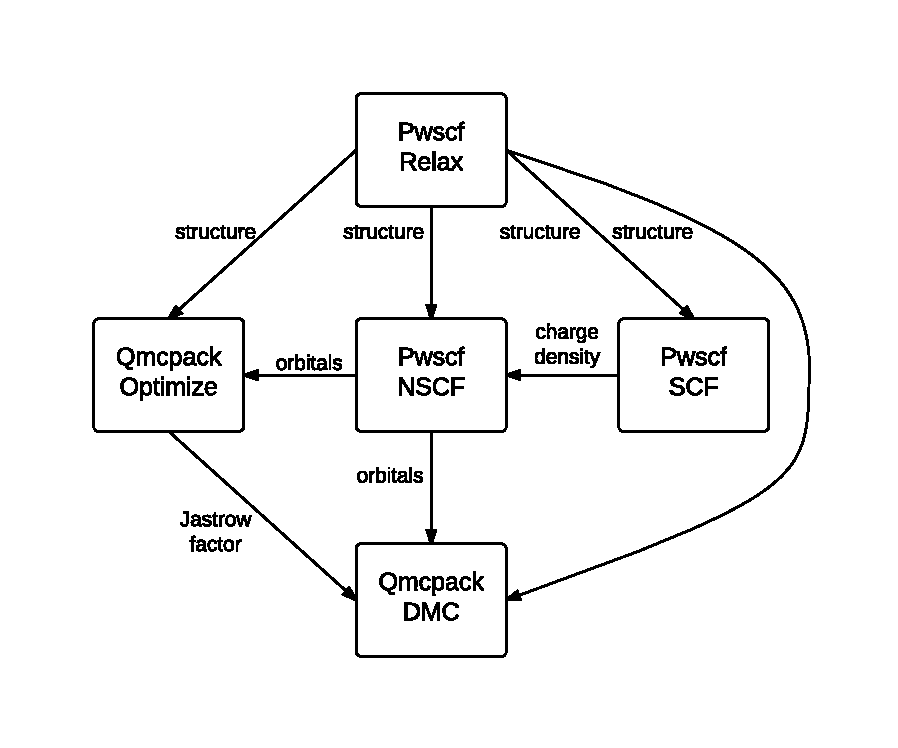
\includegraphics[trim={0 0 0 0},clip,width=\textwidth]{./figures/Nexus_workflow_example.pdf}
  \caption{An example Nexus workflow/cascade involving QMCPACK and PWSCF.  The arrows and labels denote the flow of information between the simulation runs.\label{fig:example_workflow}}
\end{figure}
\FloatBarrier


\subsection{Composing workflows from simulation objects}
Simulation workflows are created by specifying the data dependencies between simulation runs.  An example workflow is shown in Figure \ref{fig:example_workflow}.  In this case, a single relaxation calculation performed with PWSCF is providing a relaxed structure to each of the subsequent simulations.  PWSCF is used to create a converged charge density (SCF) and then orbitals at specific k-points (NSCF).  These orbitals are used by each of the two QMCPACK runs; the first optimization run provides a Jastrow factor to the final DMC run.  

Below is an example of how this workflow can be created with Nexus.  Most keywords to the \texttt{generate} functions have been omitted for brevity.  The \texttt{conv} step listed below is implicit in Figure \ref{fig:example_workflow}.
\begin{minted}{python}
relax = generate_pwscf(
    ...
    )

scf = generate_pwscf(
    dependencies = (relax,'structure'),
    ...
    )

nscf = generate_pwscf(
    dependencies = [(relax,'structure'     ),
                    (scf  ,'charge_density')],
    ...
    )

conv = generate_pw2qmcpack(
    dependencies = (nscf ,'orbitals' ),
    ...
    )

opt = generate_qmcpack(
    dependencies = [(relax,'structure'),
                    (conv ,'orbitals' )],
    ...
    )

dmc = generate_qmcpack(
    dependencies = [(relax,'structure'),
                    (conv ,'orbitals' ),
                    (opt  ,'jastrow'  )],
    ...
    )
\end{minted}

\noindent
As suggested at the beginning of this section, workflow composition logically breaks into two parts: simulation generation and workflow dependency specification.  This type of breakup can also be performed explicitly within a Nexus user script, if desired:
\begin{minted}{python}
# simulation generation
relax = generate_pwscf(...)
scf   = generate_pwscf(...)
nscf  = generate_pwscf(...)
conv  = generate_pw2qmcpack(...)
opt   = generate_qmcpack(...)
dmc   = generate_qmcpack(...)

# workflow dependency specification
scf.depends(relax,'structure')
nscf.depends((relax,'structure'     ),
             (scf  ,'charge_density'))
conv.depends(nscf ,'orbitals' )
opt.depends((relax,'structure'),
            (conv ,'orbitals' ))
dmc.depends((relax,'structure'),
            (conv ,'orbitals' ),
            (opt  ,'jastrow'  ))
\end{minted}

\noindent
More complicated workflows or scans over parameters of interest can be created with for loops and if-else logic constructs.  This is fairly straightforward to accomplish because any keyword input can given a Python variable instead of a constant, as is mostly the case in the brief examples above.



\section{Workflow execution}\label{sec:user_execution}
Simulation jobs are actually executed when the corresponding simulation objects are passed to the \texttt{run\_project} function.  Within the \texttt{run\_project} function, most of the workflow management operations unique to Nexus are actually performed.  The details of the management process is not the purpose of this section.  This process is discussed in context in the example walkthroughs (Sec. \ref{sec:examples}).

The \texttt{run\_project} function can be invoked in a couple of ways.  The most straightforward is simply to provide all simulation objects directly as arguments to this function:
\begin{minted}{python}
run_project(relax,scf,nscf,opt,dmc)
\end{minted}

\noindent
When complex workflows are being created (\textit{e.g.} when the \texttt{generate} function appear in \texttt{for} loops and \texttt{if} statements), it is generally more convenient to accumulate a list of simulation objects and then pass the list to \texttt{run\_project} as follows:
\begin{minted}{python}
sims = []

relax = generate_pwscf(...)
sims.append(relax)

scf   = generate_pwscf(...)
sims.append(scf)

nscf  = generate_pwscf(...)
sims.append(nscf)

conv  = generate_pw2qmcpack(...)
sims.append(conv)

opt   = generate_qmcpack(...)
sims.append(opt)

dmc   = generate_qmcpack(...)
sims.append(dmc)

run_project(sims)
\end{minted}

\noindent
When the \texttt{run\_project} function returns, all simulation runs should be finished.  


\section{Data analysis}\label{sec:user_data_analysis}
Following the call to \texttt{run\_project}, the user can perform data analysis tasks, if desired, as the analyzer object associated with each simulation contains a collection of post-processed output data rendered in numeric form (ints, floats, numpy arrays) and stored in a structured format.  An interactive example for QMCPACK data analysis is shown below.  Note that all analysis objects are interactively browsable in a similar manner.
\begin{shaded}
\begin{verbatim}
>>> qa=dmc.load_analyzer_image()

>>> qa.qmc
  0                     VmcAnalyzer
  1                     DmcAnalyzer
  2                     DmcAnalyzer

>>> qa.qmc[2]
  dmc                   DmcDatAnalyzer
  info                  QAinformation
  scalars               ScalarsDatAnalyzer
  scalars_hdf           ScalarsHDFAnalyzer

>>> qa.qmc[2].scalars_hdf
  Coulomb               obj
  ElecElec              obj
  Kinetic               obj
  LocalEnergy           obj
  LocalEnergy_sq        obj
  LocalPotential        obj
  data                  QAHDFdata

>>> print qa.qmc[2].scalars_hdf.LocalEnergy
  error           = 0.0201256357883
  kappa           = 12.5422841447
  mean            = -75.0484800012
  sample_variance = 0.00645881103012
  variance        = 0.850521272106
\end{verbatim}
\end{shaded}






\pagebreak
\chapter{Complete Examples} \label{sec:examples}

\bu{Disclaimer:} Please note that the examples given here do not generally qualify as production 
calculations because the supercell size, optimization process, DMC timestep and 
other key parameters may not be converged.  Pseudopotentials are provided 
``as is'' and should not be trusted without explicit validation.

Complete examples of calculations performed with Nexus are provided 
in the following sections.  These examples are intended to highlight basic 
features of Nexus and act as templates for future calculations.  
%A complete description of the available features can be found in ``Nexus 
%User Reference'' (section \ref{sec:reference}).  
If there is an example you 
would like to contribute, or if you feel an example on a particular topic is 
needed, please contact the developer at krogeljt@ornl.gov to discuss the 
possibilities.  

To perform the example calculations yourself, consult the \texttt{examples} 
directory in your Nexus installation:
\begin{shaded}
\begin{verbatim}
/your_download_path/nexus/examples
\end{verbatim}
\end{shaded}
\noindent
The examples assume that you have working versions of \texttt{pw.x}, 
\texttt{pw2qmcpack.x}, \texttt{qmcpack} (real version), and 
\texttt{qmcpack\_complex} (complex version) installed and in your \texttt{PATH}. 
A brief description of each example is given below.  


%\section{Brief example descriptions}
\begin{description}
  \item[Bulk Diamond VMC] \hfill \\
    A representative bulk calculation.  A simple workflow consisting 
    of orbital generation with PWSCF, orbital conversion with pw2qmcpack, 
    and a short VMC calculation with QMCPACK is performed.

  \item[Graphene Sheet DMC] \hfill \\
    A representative slab calculation.  The total DMC energy of a graphene 
    ``sheet'' consisting of 8 atoms is computed.  DFT is performed with 
    PWSCF on the primitive cell followed by Jastrow optimization by QMCPACK 
    and finally a supercell VMC+DMC calculation by QMCPACK.  

  \item[C 20 Molecule DMC] \hfill  \\
    A representative molecular calculation.  The total DMC energy of an ideal 
    C 20 molecule is computed.  DFT is performed with PWSCF on a periodic cell 
    with some vacuum surrounding the molecule.  QMCPACK optimization and 
    VMC+DMC follow on the system with open boundary conditions.  

    (Note that without the crystal field splitting afforded by the initial 
    artificial periodicity, the Kohn-Sham HOMO would be degenerate, and so a 
    production calculation would likely require more care in appropriately 
    setting up the wavefunction.)

  \item[Oxygen Dimer DMC] \hfill \\
    An example demonstrating automation of a simple parameter scan, in this 
    case the interparticle spacing in an oxygen dimer.  The reader will gain 
    some experience modifying Nexus user scripts to produce automated workflows.
    
  \item[Bulk Diamond Excited States VMC] \hfill \\
    A representative bulk excited states calculation.  A simple workflow consisting 
    of orbital generation with PWSCF, orbital conversion with pw2qmcpack, 
    and a short VMC calculation with QMCPACK is performed.
\end{description}





%\pagebreak
%\section{Demonstrated user script sections} \label{simple_qmc}
%The simplest QMC calculations that can be performed with Nexus 
%involve five main stages:
%\begin{description}
%  \item[Configure Nexus settings] \hfill \\
%    The \texttt{settings} function allows you to specify where pseudopotentials 
%    are located, whether to generate input files without running jobs, details 
%    of the machine you are on, and how often to have Nexus check 
%    on the status of running jobs.  \index{settings}
%
%  \item[Describe the physical system] \hfill \\
%    Generate a crystal structure with the \texttt{generate\_physical\_system} 
%    convenience function (see ``Graphene Sheet DMC'' \ref{graphene_dmc}), 
%    or load an XYZ file into a \texttt{Structure} object 
%    (see ``C 20 Molecule DMC'' \ref{c20_dmc}).  This is where 
%    information about k-points, net system charge, or net system spin are 
%    recorded.\index{generate\_physical\_system}\index{Structure}
%
%  \item[Describe simulation workflows] \hfill \\
%    Use the \texttt{standard\_qmc} (see ``Graphene Sheet DMC'' 
%    \ref{graphene_dmc}) or \texttt{basic\_qmc} (see ``C 20 Molecule DMC'' 
%    \ref{c20_dmc}) convenience functions 
%    to select specific pseudopotentials, specify PWSCF and QMCPACK input 
%    parameters, and job details, like how many nodes/cores/threads to use.
%    \index{standard\_qmc}\index{basic\_qmc}
%
%  \item[Run simulation workflows] \hfill \\
%    Pass simulation objects created by \texttt{generate\_pwscf}, 
%    \texttt{generate\_pw2qmcpack}, and \texttt{generate\_qmcpack} to 
%    Nexus through the \texttt{run\_project} function for active management.
%    \index{run\_project}
%
%  \item[Collect simulation results] \hfill \\
%    Load results of simulation objects using the \texttt{load\_analyzer\_image} 
%    function.  This gives you access to several/most (PWSCF/QMCPACK) physical 
%    results produced by the simulation with statistical analysis already 
%    performed (though the responsibility is still yours to verify absolute 
%    correctness).
%    \index{load\_analyzer\_image}
%\end{description}
%
%
%For more information about the functions/objects mentioned above, consider 
%the examples in the following sections.
%% or consult ``Nexus User Reference'' (section \ref{sec:reference}).


\pagebreak
\section{Example 1: Bulk Diamond VMC}\label{diamond_dmc}
The files for this example are found in:
\begin{shaded}
\begin{verbatim}
/your_download_path/nexus/examples/qmcpack/diamond
\end{verbatim}
\end{shaded}

By following the instructions contained in this section the reader can execute a simple workflow with Nexus.  The workflow presented here is intended to illustrate basic Nexus usage.  The example workflow has three stages: (1) orbital generation in a primitive (2 atom) cell of diamond with PWSCF, (2) conversion of the orbitals from the native PWSCF format to the ESHDF format that QMCPACK reads, and (3) a minimal variational Monte Carlo (VMC) run of a 16 atom supercell of diamond with QMCPACK.  The Nexus input script corresponding to this workflow is shown below.  

The script is similar to the one discussed in section \ref{sec:ui}, differing mainly in the name-by-name imports and the description of the physical system.  Instead of reading an external VASP POSCAR file, the structure is specified in a format native to Nexus.  The physical system is specified by providing the unit system (Angstrom in this case), the three vectors comprising the axes of the simulation cell, and the names and positions (Cartesian coordinates) of the atoms involved.  The use of ``\texttt{tiling=(2,2,2)}'' communicates the request that a $2\times2\times2$ supercell be constructed out of the specified 2 atom primitive cell.  The k-point grid applies to the supercell and is comprised of a single k-point.  The eight corresponding primitive cell images of this k-point are determined automatically by Nexus.  The text ``\texttt{C = 4}'' specifies the number of valence electrons for the carbon pseudopotential.  The pseudopotential files used in this example (\texttt{C.BFD.*}) have been adapted from an open access pseudopotential database (see \url{http://www.burkatzki.com/pseudos/index.2.html}) for use in PWSCF and QMCPACK.  Since the \texttt{PhysicalSystem} object, ``\texttt{dia16}'', contains both the supercell and its equivalent folded/primitive version, the PWSCF DFT calculation will be performed in the primitive cell to save memory for the subsequent VMC calculation of the full supercell performed with QMCPACK.

%\begin{lstlisting}[caption={Nexus input script for the usage example (\texttt{diamond.py}).  DFT is performed in diamond primitive cell followed by VMC in a 16 atom supercell.},label={ex:d16}]
\HRule
\begin{minted}{python}
#! /usr/bin/env python

# nexus imports
from nexus import settings,Job,run_project
from nexus import generate_physical_system
from nexus import generate_pwscf
from nexus import generate_pw2qmcpack
from nexus import generate_qmcpack,vmc

# general settings for nexus
settings(
    pseudo_dir    = '../pseudopotentials',# directory with all pseudopotentials
    status_only   = 0,                    # only show status of runs
    generate_only = 0,                    # only make input files
    sleep         = 3,                    # check on runs every 3 seconds
    machine       = 'ws16'                # local machine is 16 core workstation
    )

# generate diamond structure
dia16 = generate_physical_system(
    units  = 'A',                      # Angstrom units
    axes   = [[1.785,1.785,0.   ],     # cell axes
              [0.   ,1.785,1.785],
              [1.785,0.   ,1.785]],
    elem   = ['C','C'],                # 2 C atoms
    pos    = [[0.    ,0.    ,0.    ],  # atomic positions
              [0.8925,0.8925,0.8925]],
    tiling = (2,2,2),                  # tile to 16 atom cell
    kgrid  = (1,1,1),                  # single supercell k-point
    kshift = (0,0,0),                  #  at gamma
    C      = 4                         # pseudo-C (4 val. elec.)
    )
              
# scf run produces orbitals
scf = generate_pwscf(
    identifier   = 'scf',           # identifier/file prefix
    path         = 'diamond/scf',   # directory for scf run
    job          = Job(cores=16,app='pw.x'),
    input_type   = 'generic',
    calculation  = 'scf',           # perform scf calculation
    input_dft    = 'lda',           # dft functional
    ecutwfc      = 200,             # planewave energy cutoff
    conv_thr     = 1e-8,            # scf convergence threshold
    nosym        = True,            # don't use symmetry
    wf_collect   = True,            # write orbitals
    system       = dia16,           # run diamond system
    pseudos      = ['C.BFD.upf'],   # pwscf PP for C
    )

# convert orbitals for qmcpack
conv = generate_pw2qmcpack(
    identifier   = 'conv',          # identifier/file prefix
    path         = 'diamond/scf',   # directory for conv job
    job          = Job(cores=1,app='pw2qmcpack.x'),
    write_psir   = False,           # output in k-space
    dependencies = (scf,'orbitals') # get orbitals from scf
    )

# vmc run
qmc = generate_qmcpack(
    identifier   = 'vmc',           # identifier/file prefix 
    path         = 'diamond/vmc',   # directory for vmc run
    job          = Job(cores=16,threads=4,app='qmcpack'),
    input_type   = 'basic',
    system       = dia16,           # run diamond system
    pseudos      = ['C.BFD.xml'],   # qmcpack PP for C
    jastrows     = [],              # no jastrows, test run
    calculations = [
        vmc(                        # vmc inputs
            walkers     =   1,      #  one walker per core
            warmupsteps =  20,      #  20 steps before measurement
            blocks      = 200,      #  200 blocks
            steps       =  10,      #   of 10 MC steps each
            substeps    =   2,      #   2 substeps w/o measurement
            timestep    =  .4       #  0.4/Ha timestep
            )
        ],
    dependencies = (conv,'orbitals')# get orbitals from conv job
    )

# nexus monitors all runs
run_project(scf,conv,qmc)
\end{minted}
\HRule
%\end{lstlisting}


To fully execute the usage example provided here, copies of PWSCF, QMCPACK, and the orbital converter pw2qmcpack will need to be installed on the local machine.  The example assumes that the executables are in the user's \texttt{PATH} and are named \texttt{pw.x}, \texttt{qmcpack}, and \texttt{pw2qmcpack.x}.  See Sec. \ref{sec:install_code} for download and installation instructions for these codes. A test of Nexus including the generation of input files, but without actual job submission, can be performed without installing these codes.  However, Python itself and NumPy are required to run Nexus (see Sec. \ref{install_python}).    The example also assumes the local machine is a workstation with 16 available cores (``\texttt{ws16}'').  If fewer than 16 cores are available, \emph{e.g.} 4, change the example files to reflect this: \texttt{ws16}$\rightarrow$\texttt{ws4}, \texttt{Job(cores=16,$\ldots$)}$\rightarrow$\texttt{Job(cores=4,$\ldots$)}. 

In this example, we will run Nexus in three different modes:
\begin{enumerate}
  \item{status mode: print the status of each simulation and then exit (\texttt{status\_only=1}).}
  \item{generate mode: generate input files but do not execute workflows (\texttt{generate\_only=1}).}
  \item{execute mode: execute workflows by submitting jobs and monitoring simulation progress (\texttt{status\_only=0, generate\_only=0}).}
\end{enumerate}
Only the last mode requires executables for PWSCF and QMCPACK.

First, run Nexus in status mode.  Enter the \texttt{examples/qmcpack/diamond} directory, open \texttt{diamond.py} with a text editor and set ``\texttt{status\_only}=1''.  Run the script by typing ``\texttt{./diamond.py}'' at the command line and inspect the output.  The output should be similar to the text below (without the comments):
\begin{shaded}
\begin{verbatim}
       Pseudopotentials
         reading pp:  ../pseudopotentials/C.BFD.upf  # dft PP found
         reading pp:  ../pseudopotentials/C.BFD.xml  # qmc PP found
     
     Project starting 
       checking for file collisions        # files do not overlap
       loading cascade images              # load saved workflow state    
         cascade 0 checking in             # only one workflow/cascade
       checking cascade dependencies       # match producers/consumers
         all simulation dependencies satisfied 
       cascade status 
         setup, sent_files, submitted, finished, got_output, analyzed 
         000000  scf  ./runs/diamond/scf   # no work has been done yet
         000000  conv  ./runs/diamond/scf  # for any of the
         000000  vmc  ./runs/diamond/vmc   # three simulations
         setup, sent_files, submitted, finished, got_output, analyzed 
\end{verbatim}
\end{shaded}

{\flushleft
The binary string ``000000'' indicates that none of the six stages of simulation progression have been completed.  These stages correpond to the following actions/states: writing input files (``\texttt{setup}''), copying pseudopotential files (``\texttt{sent\_files}''), submitting simulation jobs for execution (``\texttt{submitted}''), the completion of a simulation job (``\texttt{finished}''), collecting output files (``\texttt{got\_output}''), and preprocessing output files for later analysis (``\texttt{analyzed}'') .  In a production setting, this mode is useful for checking the status of current workflows/cascades prior to adding new ones.  It is also useful in general for detecting any problems with the Nexus input script itself.
}

Next, run the example in generate mode.  Set ``\texttt{status\_only}=0'' and ``\texttt{generate\_only}=1'', then run the example script again.  Instead of showing workflow status, Nexus will now perform a dry run of the workflows by generating all of the run directories and input files.  The output should contain text similar to what is shown below:
\begin{shaded}
\begin{verbatim}
       starting runs:                      # start submitting jobs
       ~~~~~~~~~~~~~~~~~~~~~~~~~~~~~~ 
       poll 0  memory 60.45 MB             # first poll cycle
         Entering ./runs/diamond/scf 0     # scf job
           writing input files  0 scf      # input file written
         Entering ./runs/diamond/scf 0 
           sending required files  0 scf   # PP files copied
           submitting job  0 scf           # job is in virtual queue
         Entering ./runs/diamond/scf 0 
           Would have executed:            # shows submission command
             export OMP_NUM_THREADS=1      # does not execute
             mpirun -np 16 pw.x -input scf.in 
     
       poll 1  memory 60.72 MB 
         Entering ./runs/diamond/scf 0 
           copying results  0 scf          # output file copying stage
         Entering ./runs/diamond/scf 0 
           analyzing  0 scf                # output analysis stage
     
       poll 2  memory 60.73 MB             # third poll cycle
         Entering ./runs/diamond/scf 1     # similar for conv job
           writing input files  1 conv 
         Entering ./runs/diamond/scf 1 
           sending required files  1 conv 
           submitting job  1 conv 
         Entering ./runs/diamond/scf 1 
           Would have executed:  
             export OMP_NUM_THREADS=1
             mpirun -np 1 pw2qmcpack.x<conv.in 
     
       poll 3  memory 60.73 MB 
         Entering ./runs/diamond/scf 1 
           copying results  1 conv 
         Entering ./runs/diamond/scf 1 
           analyzing  1 conv 
     
       poll 4  memory 60.73 MB             # fifth poll cycle
         Entering ./runs/diamond/vmc 2     # similar for vmc job
           writing input files  2 vmc 
         Entering ./runs/diamond/vmc 2 
           sending required files  2 vmc 
           submitting job  2 vmc 
         Entering ./runs/diamond/vmc 2 
           Would have executed:  
             export OMP_NUM_THREADS=4
             mpirun -np 4 qmcpack vmc.in.xml 
     
       poll 5  memory 60.78 MB 
         Entering ./runs/diamond/vmc 2 
           copying results  2 vmc 
         Entering ./runs/diamond/vmc 2 
           analyzing  2 vmc 
     
     Project finished                      # jobs finished
\end{verbatim}
\end{shaded}

{\flushleft
The output describes the progress of each simulation.  The run submission commands are also clearly shown as well as the amount of memory used by Nexus.
There should now be a ``\texttt{runs}'' directory containing the generated input files with the following structure:
}
\begin{shaded}
\begin{verbatim}
          runs/
          \-- diamond               # main diamond directory
              |-- scf               #  scf directory
              |-- |-- C.BFD.upf     #   pwscf PP file
              |-- |-- conv.in       #   conv job input file
              |-- |-- pwscf_output  #   pwscf output directory
              |-- |-- scf.in        #   scf job input file
              |-- |-- sim_conv      #   nexus directory for conv
              |-- |-- |-- input.p   #    stored input object
              |-- |-- \-- sim.p     #    simulation status file
              |-- \-- sim_scf       #   nexus directory for scf
              |--     |-- input.p   #    stored input object
              |--     \-- sim.p     #    simulation status file
              \-- vmc               #  vmc directory
                  |-- C.BFD.xml     #   qmcpack PP file
                  |-- sim_vmc       #   nexus directory for vmc
                  |-- |-- input.p   #    stored input object
                  |-- \-- sim.p     #    simulation status file
                  \-- vmc.in.xml    #   vmc job input file
\end{verbatim}
\end{shaded}
{\flushleft
The ``\texttt{sim.p}'' files record the state of each simulation.  Inspect the input files generated by Nexus (\texttt{scf.in}, \texttt{conv.in}, and \texttt{vmc.in.xml}).  Compare the files with the input provided to Nexus in \texttt{diamond.py}.
}

Finally, run the example in execute mode. Remove the ``\texttt{runs}'' and ``\texttt{results}'' directories, set ``\texttt{status\_only}=0'' and ``\texttt{generate\_only}=0'', and rerun the script.  The output shown should be similar to what was seen for generate mode, only now there may be multiple workflow polls while a particular simulation is running.  The ``\texttt{sleep}'' keyword controls how often the polls occur (every 3 seconds in this example).  Note that the Nexus host process sleeps in between polls so that a minimum of computational resources are occupied.  Once ``\texttt{Project finished}'' is displayed, all the simulation runs should be complete.  Confirm the success of the runs by checking the output files.  The text ``\texttt{JOB DONE.}'' should appear near the end of the PWSCF output file \texttt{scf.out}.  QMCPACK has completed successfully if ``\texttt{Total Execution time}'' appears near the end of the output in \texttt{vmc.out}.











\pagebreak
\section{Example 2: Graphene Sheet DMC} \label{graphene_dmc}
The files for this example are found in:
\begin{shaded}
\begin{verbatim}
/your_download_path/nexus/examples/qmcpack/graphene
\end{verbatim}
\end{shaded}

Take a moment to study the ``input file'' script 
(\texttt{graphene.py}) and the attendant comments 
(prefixed with \#). 
%The five stages listed in section \ref{simple_qmc} should be apparent.


\HRule
\begin{minted}{python}
#! /usr/bin/env python

from nexus import settings,Job,run_project
from nexus import generate_physical_system
from nexus import generate_pwscf
from nexus import generate_pw2qmcpack
from nexus import generate_qmcpack
from nexus import loop,linear,vmc,dmc


# general settings for nexus
settings(
    pseudo_dir    = '../pseudopotentials',# directory with all pseudopotentials
    sleep         = 3,                    # check on runs every 'sleep' seconds
    generate_only = 0,                    # only make input files
    status_only   = 0,                    # only show status of runs
    machine       = 'ws16',               # local machine is 16 core workstation
    )



# generate the graphene physical system
graphene = generate_physical_system(
    lattice   = 'hexagonal',      # hexagonal cell shape
    cell      = 'primitive',      # primitive cell
    centering = 'P',              # primitive basis centering
    constants = (2.462,10.0),     # a,c constants
    units     = 'A',              # in Angstrom
    atoms     = ('C','C'),        # C primitive atoms
    basis     = [[ 0  , 0  , 0],  # basis vectors
                 [2./3,1./3, 0]],
    tiling    = (2,2,1),          # tiling of primitive cell
    kgrid     = (1,1,1),          # Monkhorst-Pack grid
    kshift    = (.5,.5,.5),       # and shift
    C         = 4                 # C has 4 valence electrons
    ) 


# list of simulations in workflow
sims = []

# scf run produces charge density
scf = generate_pwscf(
    # nexus inputs
    identifier   = 'scf',           # identifier/file prefix
    path         = 'graphene/scf',  # directory for scf run
    job          = Job(cores=16),   # run on 16 cores
    pseudos      = ['C.BFD.upf'],   # pwscf PP file
    system       = graphene,        # run graphene
    # input format selector
    input_type   = 'scf',           # scf, nscf, relax, or generic
    # pwscf input parameters
    input_dft    = 'lda',           # dft functional
    ecut         =  150 ,           # planewave energy cutoff (Ry)
    conv_thr     =  1e-6,           # scf convergence threshold (Ry)
    mixing_beta  =    .7,           # charge mixing factor
    kgrid        = (8,8,8),         # MP grid of primitive cell
    kshift       = (1,1,1),         #  to converge charge density
    wf_collect   = False,           # don't collect orbitals
    use_folded   = True             # use primitive rep of graphene
    )
sims.append(scf)  

# nscf run to produce orbitals for jastrow optimization
nscf_opt = generate_pwscf(
    # nexus inputs
    identifier   = 'nscf',          # identifier/file prefix      
    path         = 'graphene/nscf_opt', # directory for nscf run       
    job          = Job(cores=16),   # run on 16 cores             
    pseudos      = ['C.BFD.upf'],   # pwscf PP file               
    system       = graphene,        # run graphene                
    # input format selector                                      
    input_type   = 'nscf',          # scf, nscf, relax, or generic
    # pwscf input parameters
    input_dft    = 'lda',           # dft functional
    ecut         =  150 ,           # planewave energy cutoff (Ry)
    conv_thr     =  1e-6,           # scf convergence threshold (Ry)
    mixing_beta  =    .7,           # charge mixing factor
    nosym        = True,            # don't symmetrize k-points
    use_folded   = True,            # use primitive rep of graphene
    wf_collect   = True,            # write out orbitals
    kgrid        = (1,1,1),         # single k-point for opt
    kshift       = (0,0,0),         # gamma point
    # workflow dependencies
    dependencies = (scf,'charge_density')
    )
sims.append(nscf_opt)

# orbital conversion job for jastrow optimization
p2q_opt = generate_pw2qmcpack(
    # nexus inputs
    identifier   = 'p2q',
    path         = 'graphene/nscf_opt',
    job          = Job(cores=1),
    # pw2qmcpack input parameters
    write_psir   = False,
    # workflow dependencies
    dependencies = (nscf_opt,'orbitals')
    )
sims.append(p2q_opt)

# Jastrow optimization
opt = generate_qmcpack(
    # nexus inputs
    identifier   = 'opt',           # identifier/file prefix
    path         = 'graphene/opt',  # directory for opt run
    job          = Job(cores=16,app='qmcpack'),
    pseudos      = ['C.BFD.xml'],   # qmcpack PP file
    system       = graphene,        # run graphene
    # input format selector   
    input_type   = 'basic',
    # qmcpack input parameters
    corrections  = [], 
    jastrows     = [('J1','bspline',8),   # 1 body bspline jastrow
                    ('J2','bspline',8)],  # 2 body bspline jastrow
    calculations = [
        loop(max = 6,                        # No. of loop iterations
             qmc = linear(                   # linearized optimization method
                energy               =  0.0, # cost function
                unreweightedvariance =  1.0, #   is all unreweighted variance
                reweightedvariance   =  0.0, #   no energy or r.w. var. 
                timestep             =  0.5, # vmc timestep (1/Ha)
                warmupsteps          =  100, # MC steps before data collected 
                samples              = 16000,# samples used for cost function 
                stepsbetweensamples  =   10, # steps between uncorr. samples
                blocks               =   10, # ignore this  
                minwalkers           =   0.1,#  and this
                bigchange            =  15.0,#  and this
                alloweddifference    =  1e-4 #  and this, for now
                )
             )        
        ],
    # workflow dependencies
    dependencies = (p2q_opt,'orbitals')        
    )
sims.append(opt)


# nscf run to produce orbitals for final dmc
nscf = generate_pwscf(
    # nexus inputs
    identifier   = 'nscf',          # identifier/file prefix      
    path         = 'graphene/nscf', # directory for nscf run       
    job          = Job(cores=16),   # run on 16 cores             
    pseudos      = ['C.BFD.upf'],   # pwscf PP file               
    system       = graphene,        # run graphene                
    # input format selector                                      
    input_type   = 'nscf',          # scf, nscf, relax, or generic
    # pwscf input parameters
    input_dft    = 'lda',           # dft functional
    ecut         =  150 ,           # planewave energy cutoff (Ry)
    conv_thr     =  1e-6,           # scf convergence threshold (Ry)
    mixing_beta  =    .7,           # charge mixing factor
    nosym        = True,            # don't symmetrize k-points
    use_folded   = True,            # use primitive rep of graphene
    wf_collect   = True,            # write out orbitals
    # workflow dependencies
    dependencies = (scf,'charge_density')
    )
sims.append(nscf)

# orbital conversion job for final dmc
p2q = generate_pw2qmcpack(
    # nexus inputs
    identifier   = 'p2q',
    path         = 'graphene/nscf',
    job          = Job(cores=1),
    # pw2qmcpack input parameters
    write_psir   = False,
    # workflow dependencies
    dependencies = (nscf,'orbitals')
    )
sims.append(p2q)
    
# final dmc run
qmc = generate_qmcpack( 
    # nexus inputs
    identifier   = 'qmc',           # identifier/file prefix       
    path         = 'graphene/qmc',  # directory for dmc run       
    job          = Job(cores=16,app='qmcpack'),
    pseudos      = ['C.BFD.xml'],   # qmcpack PP file
    system       = graphene,        # run graphene
    # input format selector                                      
    input_type   = 'basic',
    # qmcpack input parameters
    corrections  = [],              # no finite size corrections
    jastrows     = [],              # overwritten from opt
    calculations = [                # qmcpack input parameters for qmc
        vmc(                        # vmc parameters 
            timestep      = 0.5,    # vmc timestep (1/Ha)
            warmupsteps   = 100,    # No. of MC steps before data is collected
            blocks        = 200,    # No. of data blocks recorded in scalar.dat
            steps         =  10,    # No. of steps per block
            substeps      =   3,    # MC steps taken w/o computing E_local
            samplesperthread = 40   # No. of dmc walkers per thread
            ),                      
        dmc(                        # dmc parameters
            timestep      = 0.01,   # dmc timestep (1/Ha)
            warmupsteps   =  50,    # No. of MC steps before data is collected
            blocks        = 400,    # No. of data blocks recorded in scalar.dat
            steps         =   5,    # No. of steps per block
            nonlocalmoves = True    # use Casula's T-moves
            ),                      #  (retains variational principle for NLPP's)
        ],
    # workflow dependencies
    dependencies = [(p2q,'orbitals'),
                    (opt,'jastrow')]
    )


# nexus monitors all runs
run_project(sims)


# print out the total energy
performed_runs = not settings.generate_only and not settings.status_only
if performed_runs:
    # get the qmcpack analyzer object
    # it contains all of the statistically analyzed data from the run
    qa = qmc.load_analyzer_image()
    # get the local energy from dmc.dat
    le = qa.dmc[1].dmc.LocalEnergy  # dmc series 1, dmc.dat, local energy
    #  print the total energy for the 8 atom system
    print 'The DMC ground state energy for graphene is:'
    print '    {0} +/- {1} Ha'.format(le.mean,le.error)
#end if
\end{minted}
\HRule

To run the example, navigate to the example directory and type
\begin{shaded}
\begin{verbatim}
./graphene.py
\end{verbatim}
\end{shaded}
or, alternatively, 
\begin{shaded}
\begin{verbatim}
python ./graphene.py
\end{verbatim}
\end{shaded}

You should see output like this (without the added \# comments):
\begin{shaded}
\begin{verbatim}
  Pseudopotentials   # reading pseudopotential files
    reading pp:  ../pseudopotentials/C.BFD.upf
    reading pp:  ../pseudopotentials/C.BFD.xml

Project starting 
  checking for file collisions  # ensure created files don't overlap
  loading cascade images        # load previous simulation state
    cascade 0 checking in 
  checking cascade dependencies # ensure sim.'s have needed dep.'s
    all simulation dependencies satisfied 
  
  starting runs:                # start submitting jobs
  ~~~~~~~~~~~~~~~~~~~~~~~~~~~~~~ 
  poll 0  memory 56.28 MB 
    Entering ./runs/graphene/scf 0      # scf job
      writing input files  0 scf        # input file written 
    Entering ./runs/graphene/scf 0 
      sending required files  0 scf     # PP files copied
      submitting job  0 scf             # job is in virtual queue
    Entering ./runs/graphene/scf 0 
      Executing:                        # job executed on workstation
        export OMP_NUM_THREADS=1
        mpirun -np 16 pw.x -input scf.in 

  poll 1  memory 56.30 MB               # waiting for job to finish
  poll 2  memory 56.30 MB 
  poll 3  memory 56.30 MB 
  poll 4  memory 56.30 MB 
    Entering ./runs/graphene/scf 0 
      copying results  0 scf            # job is finished, copy results
    Entering ./runs/graphene/scf 0 
      analyzing  0 scf                  # analyze output data

                                        # now do the same for
                                        # nscf job for Jastrow opt
                                        #   single k-point
                                        # nscf job for VMC/DMC
                                        #   multiple k-points

  poll 5  memory 56.31 MB               
    Entering ./runs/graphene/nscf 1     # nscf dmc 
      writing input files  1 nscf 
      ...
    Entering ./runs/graphene/nscfopt 4  # nscf opt 
      writing input files  4 nscf 
      ...

                                        # now convert KS orbitals
                                        # to eshdf format
                                        # with pw2qmcpack.x
                                        # for nscf opt & nscf dmc

  poll 7  memory 56.32 MB 
    Entering ./runs/graphene/nscf 2     # convert dmc orbitals
      sending required files  2 p2q 
      ...
    Entering ./runs/graphene/nscfopt 4  # convert opt orbitals
      copying results  4 nscf 
      ...

  poll 10  memory 56.32 MB 
    Entering ./runs/graphene/opt 6      # submit jastrow opt
      writing input files  6 opt        # write input file
    Entering ./runs/graphene/opt 6 
      sending required files  6 opt     # copy PP files
      submitting job  6 opt             # job is in virtual queue
    Entering ./runs/graphene/opt 6 
      Executing:                        # run qmcpack
        export OMP_NUM_THREADS=1        # w/ complex arithmetic
        mpirun -np 16 qmcpack_complex opt.in.xml 

  poll 11  memory 56.32 MB 
  poll 12  memory 56.32 MB 
  poll 13  memory 56.32 MB 
  ...
  ...
  ...
  poll 793  memory 56.32 MB   # qmcpack opt finishes
  poll 794  memory 56.32 MB   # nearly an hour later
  poll 795  memory 56.32 MB 
    Entering ./runs/graphene/opt 6 
      copying results  6 opt            # copy output files
    Entering ./runs/graphene/opt 6 
      analyzing  6 opt                  # analyze the results

  poll 796  memory 56.41 MB 
    Entering ./runs/graphene/qmc 3      # submit dmc
      writing input files  3 qmc        # write input file
    Entering ./runs/graphene/qmc 3 
      sending required files  3 qmc     # copy PP files
      submitting job  3 qmc             # job is in virtual queue
    Entering ./runs/graphene/qmc 3 
      Executing:                        # run qmcpack
        export OMP_NUM_THREADS=1
        mpirun -np 16 qmcpack_complex qmc.in.xml 

  poll 797  memory 57.31 MB 
  poll 798  memory 57.31 MB 
  poll 799  memory 57.31 MB 
  ...
  ...
  ...
  poll 1041  memory 57.31 MB   # qmcpack dmc finishes
  poll 1042  memory 57.31 MB   # about 15 minutes later
  poll 1043  memory 57.31 MB 
    Entering ./runs/graphene/qmc 3 
      copying results  3 qmc            # copy output files
    Entering ./runs/graphene/qmc 3 
      analyzing  3 qmc                  # analyze the results

Project finished                        # all jobs are finished
 
The DMC ground state energy for graphene is:
    -45.824960552 +/- 0.00498990689364 Ha    # one value from
                                             # qmcpack analyzer
\end{verbatim}
\end{shaded}

If successful, you have just performed a start-to-finish DMC calculation.  
The total energy quoted above probably will not match the one you produce 
due to different compilation environments and the probabilistic nature of 
DMC.  They should not, however differ by three sigma.

Take some time to inspect the input files generated by Nexus and 
the output files from PWSCF and QMCPACK.  The runs were performed in 
sub-directories of the \texttt{runs} directory.  The order of execution of 
the simulations is roughly \texttt{scf}, \texttt{nscf}, \texttt{nscfopt}, 
\texttt{opt}, then \texttt{qmc}.

\begin{shaded}
\begin{verbatim}
runs
└── graphene_test
    ├── nscf
    │   ├── nscf.in
    │   └── nscf.out
    ├── nscfopt
    │   ├── nscf.in
    │   └── nscf.out
    ├── opt
    │   ├── opt.in.xml
    │   └── opt.out
    ├── qmc
    │   ├── qmc.in.xml
    │   └── qmc.out
    └── scf
        ├── scf.in
        └── scf.out
\end{verbatim}
\end{shaded}

The directories above contain all the files generated by the simulations.  
Often one only wants to save the files with the most important data, which 
are generally small.  These are copied to the \texttt{results} directory 
which mirrors the structure of \texttt{runs}. 

\begin{shaded}
\begin{verbatim}
results
└── runs
    └── graphene_test
        ├── nscf
        │   ├── nscf.in
        │   └── nscf.out
        ├── nscfopt
        │   ├── nscf.in
        │   └── nscf.out
        ├── opt
        │   ├── opt.in.xml
        │   └── opt.out
        ├── qmc
        │   ├── qmc.in.xml
        │   └── qmc.out
        └── scf
            ├── scf.in
            └── scf.out
\end{verbatim}
\end{shaded}

Although this QMC run was performed at a single k-point, a twist-averaged run 
could be performed simply by changing \texttt{kgrid} in 
\texttt{generate\_physical\_system} from \texttt{(1,1,1)} to \texttt{(4,4,1)}, 
or similar.
 





\pagebreak
\section{Example 3: C 20 Molecule DMC}  \label{c20_dmc}
The files for this example are found in:
\begin{shaded}
\begin{verbatim}
/your_download_path/nexus/examples/qmcpack/c20
\end{verbatim}
\end{shaded}

Take a moment to study the ``input file'' script 
(\texttt{c20\_example.py}) and the attendant comments 
(prefixed with \#). The relevant differences from the graphene example
mostly involve how the structure is procured (it is read from an XYZ file
rather than being generated), the boundary conditions (open BC's, see 
\texttt{bconds} in the QMCPACK input parameters), and the workflow involved. 



\HRule
\begin{minted}{python}
#! /usr/bin/env python

from nexus import settings,Job,run_project
from nexus import Structure,PhysicalSystem
from nexus import generate_pwscf
from nexus import generate_pw2qmcpack
from nexus import generate_qmcpack
from nexus import loop,linear,vmc,dmc


# general settings for nexus
settings(
    pseudo_dir    = '../pseudopotentials',# directory with all pseudopotentials
    sleep         = 3,                    # check on runs every 'sleep' seconds
    generate_only = 0,                    # only make input files
    status_only   = 0,                    # only show status of runs
    machine       = 'ws16',               # local machine is 16 core workstation
    )


#generate the C20 physical system
# specify the xyz file
structure_file = 'c20.cage.xyz'
# make an empty structure object
structure = Structure()
# read in the xyz file
structure.read_xyz(structure_file)
# place a bounding box around the structure
structure.bounding_box(
    box   = 'cubic',         # cube shaped cell
    scale = 1.5              # 50% extra space
    )
# make it a gamma point cell
structure.add_kmesh(
    kgrid      = (1,1,1),    # Monkhorst-Pack grid
    kshift     = (0,0,0)     # and shift
    )
# add electronic information
c20 = PhysicalSystem(
    structure = structure,   # C20 structure
    net_charge = 0,          # net charge in units of e
    net_spin   = 0,          # net spin in units of e-spin
    C          = 4           # C has 4 valence electrons
    ) 


# list of simulations in workflow
sims = []

# scf run produces charge density
scf = generate_pwscf(
    # nexus inputs
    identifier   = 'scf',           # identifier/file prefix
    path         = 'c20/scf',       # directory for scf run
    job          = Job(cores=16),   # run on 16 cores
    pseudos      = ['C.BFD.upf'],   # pwscf PP file
    system       = c20,             # run c20
    # input format selector
    input_type   = 'scf',           # scf, nscf, relax, or generic
    # pwscf input parameters
    input_dft    = 'lda',           # dft functional
    ecut         =  150 ,           # planewave energy cutoff (Ry)
    conv_thr     =  1e-6,           # scf convergence threshold (Ry)
    mixing_beta  =    .7,           # charge mixing factor
    nosym        = True,            # don't use symmetry
    wf_collect   = True,            # write out orbitals
    )
sims.append(scf)  

# orbital conversion job for opt and dmc
p2q = generate_pw2qmcpack(
    # nexus inputs
    identifier   = 'p2q',
    path         = 'c20/nscf',
    job          = Job(cores=1),
    # pw2qmcpack input parameters
    write_psir   = False,
    # workflow dependencies
    dependencies = (scf,'orbitals')
    )
sims.append(p2q)


# Jastrow optimization
opt = generate_qmcpack(
    # nexus inputs
    identifier   = 'opt',           # identifier/file prefix
    path         = 'c20/opt',       # directory for opt run
    job          = Job(cores=16,app='qmcpack'),
    pseudos      = ['C.BFD.xml'],   # qmcpack PP file
    system       = c20,             # run c20
    # input format selector   
    input_type   = 'basic',
    # qmcpack input parameters
    corrections  = [], 
    jastrows     = [('J1','bspline',8,6),   # 1 body bspline jastrow
                    ('J2','bspline',8,8)],  # 2 body bspline jastrow
    calculations = [
        loop(max = 6,                        # No. of loop iterations
             qmc = linear(                   # linearized optimization method
                energy               =  0.0, # cost function
                unreweightedvariance =  1.0, #   is all unreweighted variance
                reweightedvariance   =  0.0, #   no energy or r.w. var. 
                timestep             =  0.5, # vmc timestep (1/Ha)
                warmupsteps          =  100, # MC steps before data collected 
                samples              = 16000,# samples used for cost function 
                stepsbetweensamples  =   10, # steps between uncorr. samples
                blocks               =   10, # ignore this  
                minwalkers           =   0.1,#  and this
                bigchange            =  15.0,#  and this
                alloweddifference    =  1e-4 #  and this, for now
                )
             )        
        ],
    # workflow dependencies
    dependencies = (p2q,'orbitals')        
    )
sims.append(opt)

    
# final dmc run
qmc = generate_qmcpack( 
    # nexus inputs
    identifier   = 'qmc',           # identifier/file prefix       
    path         = 'c20/qmc',  # directory for dmc run       
    job          = Job(cores=16,app='qmcpack'),
    pseudos      = ['C.BFD.xml'],   # qmcpack PP file
    system       = c20,             # run c20
    # input format selector                                      
    input_type   = 'basic',
    # qmcpack input parameters
    corrections  = [],              # no finite size corrections
    jastrows     = [],              # overwritten from opt
    calculations = [                # qmcpack input parameters for qmc
        vmc(                        # vmc parameters 
            timestep      = 0.5,    # vmc timestep (1/Ha)
            warmupsteps   = 100,    # No. of MC steps before data is collected
            blocks        = 200,    # No. of data blocks recorded in scalar.dat
            steps         =  10,    # No. of steps per block
            substeps      =   3,    # MC steps taken w/o computing E_local
            samplesperthread = 40   # No. of dmc walkers per thread
            ),                      
        dmc(                        # dmc parameters
            timestep      = 0.01,   # dmc timestep (1/Ha)
            warmupsteps   =  50,    # No. of MC steps before data is collected
            blocks        = 400,    # No. of data blocks recorded in scalar.dat
            steps         =   5,    # No. of steps per block
            nonlocalmoves = True    # use Casula's T-moves
            ),                      #  (retains variational principle for NLPP's)
        ],
    # workflow dependencies
    dependencies = [(p2q,'orbitals'),
                    (opt,'jastrow')]
    )



# nexus monitors all runs
run_project(sims)



# print out the total energy
performed_runs = not settings.generate_only and not settings.status_only
if performed_runs:
    # get the qmcpack analyzer object
    # it contains all of the statistically analyzed data from the run
    qa = qmc.load_analyzer_image()
    # get the local energy from dmc.dat
    le = qa.dmc[1].dmc.LocalEnergy  # dmc series 1, dmc.dat, local energy
    #  print the total energy for the 20 atom system
    print 'The DMC ground state energy for C20 is:'
    print '    {0} +/- {1} Ha'.format(le.mean,le.error)
#end if
\end{minted}
\HRule


To run the example, navigate to the example directory and type
\begin{shaded}
\begin{verbatim}
./c20.py
\end{verbatim}
\end{shaded}
or, alternatively, 
\begin{shaded}
\begin{verbatim}
python ./c20.py
\end{verbatim}
\end{shaded}

You should see output like this (without the added \# comments):
\begin{shaded}
\begin{verbatim}
  Pseudopotentials   # reading pseudopotential files
    reading pp:  ../pseudopotentials/C.BFD.upf
    reading pp:  ../pseudopotentials/C.BFD.xml

Project starting 
  checking for file collisions  # ensure created files don't overlap 
  loading cascade images        # load previous simulation state 
    cascade 0 checking in 
  checking cascade dependencies # ensure sim.'s have needed dep.'s
    all simulation dependencies satisfied 
  
  starting runs:                # start submitting jobs
  ~~~~~~~~~~~~~~~~~~~~~~~~~~~~~~
  poll 0  memory 56.21 MB 
    Entering ./runs/c20/scf 0       # scf job
      writing input files  0 scf    # input file written
    Entering ./runs/c20/scf 0 
      sending required files  0 scf # PP files copied
      submitting job  0 scf         # job is in the virtual queue
    Entering ./runs/c20/scf 0 
      Executing:                    # job executed on workstation
        export OMP_NUM_THREADS=1
        mpirun -np 16 pw.x -input scf.in 

  poll 1  memory 56.23 MB           # waiting for job to finish
  poll 2  memory 56.23 MB 
  poll 3  memory 56.23 MB 
  poll 4  memory 56.23 MB 
  poll 5  memory 56.23 MB 
  poll 6  memory 56.23 MB 
  poll 7  memory 56.23 MB 
  poll 8  memory 56.23 MB 
    Entering ./runs/c20/scf 0 
      copying results  0 scf        # job is finished, copy results
    Entering ./runs/c20/scf 0 
      analyzing  0 scf              # analyze output data
                                    
  poll 9  memory 56.23 MB           # now convert KS orbitals
    Entering ./runs/c20/scf 1       # to eshdf format
      writing input files  1 p2q    # with pw2qmcpack.x
      ...

  poll 12  memory 56.23 MB 
    Entering ./runs/c20/opt 3       # submit jastrow opt
      writing input files  3 opt    # write input file
    Entering ./runs/c20/opt 3 
      sending required files  3 opt # copy PP files
      submitting job  3 opt         # job is in virtual queue
    Entering ./runs/c20/opt 3 
      Executing:                    # run qmcpack
        export OMP_NUM_THREADS=1    # w/ real arithmetic
        mpirun -np 16 qmcpack opt.in.xml 

  poll 13  memory 56.24 MB 
  poll 14  memory 56.24 MB 
  poll 15  memory 56.24 MB 
  ...
  ...
  ...
  poll 204  memory 56.24 MB   # qmcpack opt finishes
  poll 205  memory 56.24 MB   # about 10 minutes later
  poll 206  memory 56.24 MB 
    Entering ./runs/c20/opt 3 
      copying results  3 opt        # copy output files
    Entering ./runs/c20/opt 3 
      analyzing  3 opt              # analyze the results

  poll 207  memory 56.27 MB 
    Entering ./runs/c20/qmc 2       # submit dmc
      writing input files  2 qmc    # write input file
    Entering ./runs/c20/qmc 2 
      sending required files  2 qmc # copy PP files
      submitting job  2 qmc         # job is in virtual queue
    Entering ./runs/c20/qmc 2 
      Executing:                    # run qmcpack
        export OMP_NUM_THREADS=1
        mpirun -np 16 qmcpack qmc.in.xml 

  poll 208  memory 56.49 MB 
  poll 209  memory 56.49 MB 
  poll 210  memory 56.49 MB 
  ...
  ...
  ...
  poll 598  memory 56.49 MB   # qmcpack dmc finishes
  poll 599  memory 56.49 MB   # about 20 minutes later
  poll 600  memory 56.49 MB 
    Entering ./runs/c20/qmc 2 
      copying results  2 qmc        # copy output files
    Entering ./runs/c20/qmc 2 
      analyzing  2 qmc              # analyze the results

Project finished                    # all jobs are finished
 
The DMC ground state energy for C20 is:
    -112.890695404 +/- 0.0151688786226 Ha  # one value from
                                           # qmcpack analyzer
\end{verbatim}
\end{shaded}

Again, the total energy quoted above probably will not match the one you produce 
due to different compilation environments and the probabilistic nature of 
QMC.  The results should still be statistically comparable.

The directory trees generated by Nexus for C 20 have a similar structure 
to the graphene example.  Note the absence of the \texttt{nscf} runs.  The order 
of execution of the simulations is \texttt{scf}, \texttt{opt}, then \texttt{qmc}.

\begin{shaded}
\begin{verbatim}
runs
└── c20_test
    ├── opt
    │   ├── opt.in.xml
    │   └── opt.out
    ├── qmc
    │   ├── qmc.in.xml
    │   └── qmc.out
    └── scf
        ├── scf.in
        └── scf.out
results
└── runs
    └── c20_test
        ├── opt
        │   ├── opt.in.xml
        │   └── opt.out
        ├── qmc
        │   ├── qmc.in.xml
        │   └── qmc.out
        └── scf
            ├── scf.in
            └── scf.out
\end{verbatim}
\end{shaded}





\pagebreak
\section{Example 4: Automated oxygen dimer binding curve}
The files for this example are found in:
\begin{shaded}
\begin{verbatim}
/your_download_path/nexus/examples/qmcpack/oxygen_dimer
\end{verbatim}
\end{shaded}

Enter the \texttt{examples/qmcpack/oxygen\_dimer} directory.  Open \texttt{oxygen\_dimer.py} with a text editor.  The overall format is similar to the example file shown in the prior sections.  The header material, including Nexus imports, settings, and the job parameters for QMC are nearly identical.  
%The main difference is that optimization and DMC runs are being performed rather than a single VMC run.  

Following the job parameters, inputs for the optimization method are given.  The keywords are identical to the parameters of QMCPACK's XML input file.
\begin{minted}{python}
linopt1 = linear(
    energy               = 0.0,
    unreweightedvariance = 1.0,
    reweightedvariance   = 0.0,
    timestep             = 0.4,
    samples              = 5000, 
    warmupsteps          = 50,
    blocks               = 200,
    substeps             = 1,
    nonlocalpp           = True,
    usebuffer            = True,
    walkers              = 1,
    minwalkers           = 0.5,
    maxweight            = 1e9,
    usedrift             = True,
    minmethod            = 'quartic',
    beta                 = 0.025,
    exp0                 = -16,
    bigchange            = 15.0,
    alloweddifference    = 1e-4,
    stepsize             = 0.2,
    stabilizerscale      = 1.0,
    nstabilizers         = 3
    )
\end{minted}
\noindent
Requesting multiple loop's with different numbers of samples is more compact than in the native XML input file:
\begin{minted}{python}
linopt1 = ...

linopt2 = linopt1.copy()  
linopt2.samples = 20000 # opt w/ 20000 samples

linopt3 = linopt1.copy()
linopt3.samples = 40000 # opt w/ 40000 samples

opt_calcs = [loop(max=8,qmc=linopt1), # loops over opt's
             loop(max=6,qmc=linopt2),
             loop(max=4,qmc=linopt3)]
\end{minted}
\noindent
The VMC/DMC method inputs also mirror the XML:
\begin{minted}{python}
qmc_calcs = [
    vmc(
        walkers     =   1,
        warmupsteps =  30,
        blocks      =  20,
        steps       =  10,
        substeps    =   2,
        timestep    =  .4,
        samples     = 2048
        ),
    dmc(
        warmupsteps   = 100, 
        blocks        = 400,
        steps         =  32,
        timestep      = 0.01,
        nonlocalmoves = True
        )
    ]
\end{minted}
\noindent
As in the prior examples, the oxygen dimer is generated with the \texttt{generate\_physical\_system} function:
\begin{minted}{python}
dimer = generate_physical_system(
    type       = 'dimer',
    dimer      = ('O','O'),
    separation = 1.2074*scale,
    Lbox       = 15.0,
    units      = 'A',
    net_spin   = 2,
    O          = 6
    )
\end{minted}
\noindent
Similar syntax can be used to generate crystal structures or to specify systems with arbitrary atomic configurations and simulation cells.  Notice that a ``\texttt{scale}'' variable has been introduced to stretch or compress the dimer.  

Next, objects representing DFT calculations and orbital conversions are constructed with the \texttt{generate\_pwscf} and \texttt{generate\_pw2qmcpack} functions.
\begin{minted}{python}
scf = generate_pwscf(
    identifier   = 'scf',
    ...
    )
sims.append(scf)

p2q = generate_pw2qmcpack(
    identifier   = 'p2q',
    ...
    dependencies = (scf,'orbitals')
    )
sims.append(p2q)
\end{minted}

Finally, objects representing QMCPACK simulations are constructed with the \texttt{generate\_qmcpack} function:
\begin{minted}{python}
opt = generate_qmcpack(
    identifier   = 'opt',
    ...
    jastrows     = [('J1','bspline',8,4.5), 
                    ('J2','pade',0.5,0.5)],
    calculations = opt_calcs,
    dependencies = (p2q,'orbitals')
    )
sims.append(opt)

qmc = generate_qmcpack(
    identifier   = 'qmc',
    ...
    jastrows     = [],            
    calculations = qmc_calcs,
    dependencies = [(p2q,'orbitals'),
                    (opt,'jastrow')]
    )
sims.append(qmc)
\end{minted}
\noindent
Shared details such as the run directory, job, pseudopotentials, and orbital file have been omitted (\texttt{...}).  The ``\texttt{opt}'' run will optimize a 1-body B-spline Jastrow with 8 knots having a cutoff of 4.5 Bohr and a 2-body Pad\'{e} Jastrow with up-up and up-down ``\texttt{B}'' parameters set to 0.5 1/Bohr.  The Jastrow list for the DMC run is empty and a new keyword is present: \texttt{dependencies}.  The usage of \texttt{dependencies} above indicates that the DMC run depends on the optimization run for the Jastrow factor.  Nexus will submit the ``\texttt{opt}'' run first and upon completion it will scan the output, select the optimal set of parameters, pass the Jastrow information to the ``\texttt{qmc}'' run and then submit the DMC job.  Independent job workflows are submitted in parallel when permitted.  No input files are written or job submissions made until the ``\texttt{run\_project}'' function is reached.

As written, \texttt{oxygen\_dimer.py} will only perform calculations at the equilibrium separation distance of 1.2074 Angstrom.  Modify the file now to perform DMC calculations across a range of separation distances with each DMC run using the Jastrow factor optimized at the equilibrium separation distance.  The necessary Python \texttt{for} loop syntax should look something like this:
\begin{minted}{python}
sims = []
for scale in [1.00,0.90,0.95,1.05,1.10]:
    ...
    dimer = ...
    if scale==1.00:
        opt = ...
        ...
    #end if
    qmc = ...
    ...
#end for
run_project(sims)
\end{minted}
\noindent
Note that the text inside the \texttt{for} loop and the \texttt{if} block must be indented by precisely four spaces.  If you use Emacs, changes in indentation can be performed easily with \texttt{Cntrl-C >} and \texttt{Cntrl-C <} after highlighting a block of text (other editors should have similar functionality).  

Change the ``\texttt{status\_only}'' parameter in the ``\texttt{settings}'' function to \texttt{1} and type ``./oxygen\_dimer.py'' at the command line.  This will print the status of all simulations:
\begin{shaded}
\begin{verbatim}
Project starting 
  checking for file collisions 
  loading cascade images 
    cascade 0 checking in 
  checking cascade dependencies 
    all simulation dependencies satisfied 
  cascade status 
    setup, sent_files, submitted, finished, got_output, analyzed 
    000000  scf  ./scale_1.0 
    000000  scf  ./scale_0.9 
    000000  scf  ./scale_0.95 
    000000  scf  ./scale_1.05 
    000000  scf  ./scale_1.1 
    000000  p2q  ./scale_1.0 
    000000  p2q  ./scale_0.9 
    000000  p2q  ./scale_0.95 
    000000  p2q  ./scale_1.05 
    000000  p2q  ./scale_1.1 
    000000  opt  ./scale_1.0 
    000000  qmc  ./scale_1.0 
    000000  qmc  ./scale_0.9 
    000000  qmc  ./scale_0.95 
    000000  qmc  ./scale_1.05 
    000000  qmc  ./scale_1.1 
    setup, sent_files, submitted, finished, got_output, analyzed 
\end{verbatim}
\end{shaded}
\noindent
In this case, a single independent simulation ``cascade'' (workflow) has been identified, containing one ``\texttt{opt}'' and five dependent ``\texttt{qmc}'' runs.  The six status flags (\texttt{setup}, \texttt{sent\_files}, \texttt{submitted}, \texttt{finished}, \texttt{got\_output}, \texttt{analyzed}) each show \texttt{0}, indicating that no work has been done yet.  

Now change ``\texttt{status\_only}'' back to \texttt{0}, set ``\texttt{generate\_only}'' to \texttt{1}, and run \texttt{oxygen\_dimer.py} again.  This will perform a dry-run of all simulations.  The dry-run should finish in about 20 seconds:
\begin{shaded}
\begin{verbatim}
Project starting 
  checking for file collisions 
  loading cascade images 
    cascade 0 checking in 
  checking cascade dependencies 
    all simulation dependencies satisfied 
  
  starting runs:
  ~~~~~~~~~~~~~~~~~~~~~~~~~~~~~~ 
  poll 0  memory 88.54 MB 
    Entering ./scale_1.0 0 
      writing input files  0 opt 
    Entering ./scale_1.0 0 
      sending required files  0 opt 
      submitting job  0 opt 
    Entering ./scale_1.0 1 
      Would have executed:  qsub --mode script --env BG_SHAREDMEMSIZE=32 opt.qsub.in 

  poll 1  memory 88.54 MB 
    Entering ./scale_1.0 0 
      copying results  0 opt 
    Entering ./scale_1.0 0 
      analyzing  0 opt 

  poll 2  memory 88.87 MB 
    Entering ./scale_1.0 1 
      writing input files  1 qmc 
    Entering ./scale_1.0 1 
      sending required files  1 qmc 
      submitting job  1 qmc 
    ...
    Entering ./scale_1.0 2 
      Would have executed:  qsub --mode script --env BG_SHAREDMEMSIZE=32 qmc.qsub.in 
    ...

Project finished
\end{verbatim}
\end{shaded}
\noindent
Nexus polls the simulation status every 3 seconds and sleeps in between.  The ``scale\_*'' directories should now contain several files:
\begin{shaded}
\begin{verbatim}
scale_1.0
├── O2.pwscf.h5
├── O.BFD.xml
├── opt.in.xml
├── opt.qsub.in
├── qmc.in.xml
├── qmc.qsub.in
├── sim_opt
│   ├── analyzer.p
│   ├── input.p
│   └── sim.p
└── sim_qmc
    ├── analyzer.p
    ├── input.p
    └── sim.p
\end{verbatim}
\end{shaded}
\noindent
Take a minute to inspect the generated input (\texttt{opt.in.xml}, \texttt{qmc.in.xml}) and submission (\texttt{opt.qsub.in}, \texttt{qmc.qsub.in}) files.  The pseudopotential file \texttt{O.BFD.xml} has been copied into each local directory. Two additional directories have been created: \texttt{sim\_opt} and \texttt{sim\_qmc}.  The \texttt{sim.p} files in each directory contain the current status of each simulation.  If you run \texttt{oxygen\_dimer.py} again, it should not attempt to rerun any of the simulations:   
\begin{shaded}
\begin{verbatim}
Project starting 
  checking for file collisions 
  loading cascade images 
    cascade 0 checking in 
    cascade 8 checking in 
    cascade 2 checking in 
    cascade 4 checking in 
    cascade 6 checking in 
  checking cascade dependencies 
    all simulation dependencies satisfied 
  
  starting runs:
  ~~~~~~~~~~~~~~~~~~~~~~~~~~~~~~ 
  poll 0  memory 60.10 MB 
Project finished
\end{verbatim}
\end{shaded}
\noindent
This way one can continue to add to the \texttt{oxygen\_dimer.py} file (\emph{e.g.} adding more separation distances) without worrying about duplicate job submissions.

Now actually submit the optimization and DMC jobs.  Reset the state of the simulations by removing the \texttt{sim.p} files (``\texttt{rm ./scale*/sim*/sim.p}''), set ``\texttt{generate\_only}'' to \texttt{0}, and rerun \texttt{oxygen\_dimer.py}.  It should take about 15 minutes for all the jobs to complete.  You may wish to open another terminal to monitor the progress of the individual jobs while the current terminal runs \texttt{oxygen\_dimer.py} in the foreground.  

After completion, try expanding to the full set of ``\texttt{scale}'' values:\newline \texttt{[0.90,0.925,0.95,0.975,1.00,1.025,1.05,1.075,1.10]}.  Nexus should only run the workflows that correspond to new values.  In this way, Nexus scripts can be expanded over time to include new aspects of growing projects. 


\section{Example 5: Bulk Diamond Excited States VMC}\label{excited}
\section{Example 5: Bulk Diamond Excited States VMC}\label{excited}
The files for this example are found in:
\begin{shaded}
\begin{verbatim}
/your_download_path/nexus/examples/qmcpack/excited
\end{verbatim}
\end{shaded}

Please study Lab 5 in QMCPACK manual for an in-depth discussion of the excited states calculations. The primitive cell for a structure is not unique, therefore it must be standardized to generate reproducible Brillouin zones (BZ). For this end, we use "SeeK-Path" python libraries to generate standardized primitive cells and generate band structure paths. Therefore, SeeK-Path libraries must be installed using "pip install seekpath", prior to running scripts in this example. 
In this example, input file script "vmc.py" is identical to "optical.py" in Lab5 of the QMCPACK manual. 

We use neutral primitive cells at the wavefunction generation. However, creation / annihilation operations are applied at VMC level to simulate optical excitations. Compared to the ground state bulk calculations, a tiling matrix that is commensurate with the wavevectors involved in the excitation must be chosen. This process has been automatized in Nexus using the "get\_band\_tiling" function. There are two VMC scripts in this lab: \texttt{vmc.py} script uses a non-optimal tiling matrix from Lab 5 in QMCPACK, whereas \texttt{vmc-opt-tiling.py} uses the  "get\_band\_tiling" function. In this example, we will use \texttt{vmc-opt-tiling.py}. 

In Lab5 of the QMCPACK manual we found that VBM is located at $\Gamma$ and the CBM is located at $\Delta$ ([0.377, 0., 0.377]), hence C-diamond is an indirect band gap material. However, studying this transition at the given exact points would involve a very large simulation cell. Therefore, we try to round $\Delta$ to the nearest fraction with integer denominator. Tolerance of this rounding procedure is controlled by "max\_volfac" keyword in the "get\_band\_tiling" function. "max\_volfac" basically controls the maximum volume factor of the supercell being searched, which inherently controls the highest k-point grid density in one dimension. 

In the "qmc" object given below, pay attention to keyword "excitation   = ['up', '0 3 1 4']". Value for the excitation keyword can be given in list or tuple format. Here, first element of the list ('up') denotes the spin channel used to perform the excitation. Whereas '0 3 1 4' denotes the twist-index (ti) and band-index (bi) of annihilation and creation (an/cr) operations in $ti_{an} bi_{an} ti_{cr} bi_{cr}$ format. Another option is to use an indexing of the orbitals depending on their energetic ordering. In this example this would correspond to "excitation   = ['up', '-11 +12']". Band/twist index and energy indexes of the orbitals can be found in "einspline" files or they can be determined after parsing the "nscf.out" file using PwscfAnalyzer. Examples on how to do are provided in Lab 5 of the QMCPACK manual.\\
%\begin{lstlisting}[caption={Nexus input script for the usage example (\texttt{diamond.py}).  DFT is performed in diamond primitive cell followed by VMC in a 16 atom supercell.},label={ex:d16}]
\HRule
\begin{minted}{python}
#! /usr/bin/env python

from nexus import settings,job,run_project
from nexus import generate_physical_system
from nexus import generate_pwscf
from nexus import generate_pw2qmcpack
from nexus import generate_qmcpack,vmc
from structure import *

settings(
    pseudo_dir    = '../pseudopotentials',
    status_only   = 0,
    generate_only = 0,
    sleep         = 3,
    machine       = 'ws16'
    )

#Input structure
dia = generate_physical_system(
    units  = 'A',
    axes   = [[ 1.785,  1.785,  0.   ],
              [ 0.   ,  1.785,  1.785],
              [ 1.785,  0.   ,  1.785]],
    elem   = ['C','C'],
    pos    = [[ 0.    ,  0.    ,  0.    ],
              [ 0.8925,  0.8925,  0.8925]],
    C      = 4
    )

# Standardized Primitive cell -- run rest of the calculations on this cell
dia2_structure   = get_primitive_cell(structure=dia.structure)['structure']
# get_band_tiling and get_primitiev_cell require "SeeK-path" python libraries

# Returns commensurate optimum tiling matrix for the kpoints_rel wavevectors
# max_volfac is default to 20
tiling = get_band_tiling(structure   = dia2_structure,
                         kpoints_rel = [[0.000, 0.000, 0.000],
                                        [0.3768116, 0.,        0.3768116]])
# Numerical value for the second wavevector can be different in different computers, 
# adjust accordingly

# All wavevectors must be on the iBZ k_path! (get_kpath output in band.py)

# K-points can also be defined using their labels 
# (for high symmetry k-points only). For example:
# tiling = get_band_tiling(structure   = dia2_structure,
#                         kpoints_label = ['GAMMA', 'X'])

dia2 = generate_physical_system(
    structure    = dia2_structure,
    kgrid  = (1,1,1),
    kshift = (0,0,0), # Assumes we study transitions from Gamma. 
    #For non-gamma tilings, use kshift appropriately
    tiling = tiling,
    C            = 4,
    )

scf = generate_pwscf(
    identifier   = 'scf',
    path         = 'diamond/scf',
    job          = job(nodes=1, app='pw.x',hours=1),
    input_type   = 'generic',
    calculation  = 'scf',
    nspin        = 2,
    input_dft    = 'lda',
    ecutwfc      = 200,
    conv_thr     = 1e-8,
    nosym        = True,
    wf_collect   = True,
    system       = dia2,
    tot_magnetization = 0,
    pseudos      = ['C.BFD.upf'],
    )

nscf = generate_pwscf(
    identifier   = 'nscf',
    path         ='diamond/nscf_opt_tiling',
    job          = job(nodes=1, app='pw.x',hours=1),
    input_type   = 'generic',
    calculation  = 'nscf',
    input_dft    = 'lda',
    ecutwfc      = 200,
    nspin        = 2,
    conv_thr     = 1e-8,
    nosym        = True,
    wf_collect   = True,
    system       = dia2,
    nbnd         = 8,      #a sensible nbnd value can be given
    verbosity    = 'high', #verbosity must be set to high
    pseudos      = ['C.BFD.upf'],
    dependencies = (scf, 'charge_density'),
)

conv = generate_pw2qmcpack(
    identifier   = 'conv',
    path         = 'diamond/nscf_opt_tiling',
    job          = job(cores=1,app='pw2qmcpack.x',hours=1),
    write_psir   = False,
    dependencies = (nscf,'orbitals'),
    )

qmc = generate_qmcpack(
    det_format     = 'old',
    identifier     = 'vmc',
    path           = 'diamond/vmc_opt_tiling',
    job            = job(cores=16,threads=16,app='qmcpack',hours = 1),
    input_type     = 'basic',
    spin_polarized = True,
    system         = dia2,
    pseudos        = ['C.BFD.xml'],
    jastrows       = [],
    calculations   = [
        vmc(
            walkers     =  16,
            warmupsteps =  20,
            blocks      = 1000,
            steps       =  10,
            substeps    =   2,
            timestep    =  .4
            )
        ],
    dependencies = (conv,'orbitals'),
    )

qmc_optical = generate_qmcpack(
    det_format     = 'old',
    identifier     = 'vmc',
    path           = 'diamond/vmc_opt_tiling_optical',
    job            = job(cores=16,threads=16,app='qmcpack',hours = 1),
    input_type     = 'basic',
    spin_polarized = True,
    system         = dia2,
    excitation     = ['up', '0 3 1 4'], #
    pseudos        = ['C.BFD.xml'],
    jastrows       = [],
    calculations   = [
        vmc(
            walkers     =  16,
            warmupsteps =  20,
            blocks      = 1000,
            steps       =  10,
            substeps    =   2,
            timestep    =  .4
            )
        ],
    dependencies = (conv,'orbitals'),
    )

run_project(scf,nscf,conv,qmc)

\end{minted}
\HRule
















%\pagebreak
%\chapter{Nexus User Reference} \label{sec:reference}
%Pending.
%
%
%\subsection{\bu{Accessing settings data}}
%
%
%
%\section{Making structures}
%
%\section{Making simulations}
%
%\section{Linking simulations together in cascades}
%
%
%
%\section{Working with objects}
%\subsection{\bu{General properties of objects}}
%At a conceptual level, objects are a generalization of normal variables.  
%They are really collections of variables taking integer, real, string, or 
%even object values.  An object is also more than structured data, as it 
%makes available operations, or functions, that act on that data.  The data 
%(member data) and functions (member functions) of an object are accessed with 
%a ``.'' following the object's name.  So when you see code like
%\begin{shaded}
%\begin{verbatim}
%   from mymod import MyObj  # make MyObj available from the mymod module
%   i = 5                    # make an integer
%   s = 'abc'                # make a string
%   o = MyObj()              # make a MyObj called o
%   j = i + o.an_int         # access member data an_int, created with MyObj() 
%   r = o.create_real()      # access member function create_real
%   o.a = i                  # create a new member data field called a
%   take_action(             # a normal function call
%      a = 3,                #   with keyword arguments
%      i = i,                #   left i is argument, right i is variable above
%      more = True           #   and more function arguments
%      )                     #   closing the function call ()
%\end{verbatim}
%\end{shaded}
%it should be clear what is happening.
%
%\subsection{\bu{Interacting with Nexus objects}}
%All objects in Nexus behave and can be interacted with in a 
%similar way.  Each object you encounter that is made by Nexus 
%can be used in the same way as \texttt{obj} objects from the \texttt{generic} 
%module
%
%
%\section{Objects describing matter}
%\subsection{\bu{Structure}}
%\subsection{\bu{PhysicalSystem}}
%
%
%\section{Objects describing simulations}
%\subsection{\bu{General properties of \texttt{Simulation} objects}}
%\subsection{\bu{Sqd}}
%\subsection{\bu{Pwscf}}
%\subsection{\bu{Pw2casino}}
%\subsection{\bu{Pw2qmcpack}}
%\subsection{\bu{Wfconvert}}
%\subsection{\bu{Qmcpack}}
%
%
%\section{Objects describing simulation input files}
%\subsection{\bu{SqdInput}}
%\subsection{\bu{PwscfInput}}
%\subsection{\bu{Pw2casinoInput}}
%\subsection{\bu{Pw2qmcpackInput}}
%\subsection{\bu{WfconvertInput}}
%\subsection{\bu{QmcpackInput}}
%
%
%\section{Objects describing machines}
%\subsection{\bu{Workstation}}
%\subsection{\bu{Supercomputer} }
%
%
%\section{Objects describing/affecting jobs and job submission}
%\subsection{\bu{Job}}
%\subsection{\bu{bundle}}
%\subsection{\bu{ProjectManager}}
%
%
%\section{Objects and functions for data analysis}
%\subsection{\bu{Unit conversion: convert}}
%\subsection{\bu{PWCSF data analysis: PwscfAnalyzer}}
%\subsection{\bu{QMCPACK data analysis: QmcpackAnalyzer}}
%\subsection{\bu{Fitting equation of state data: eos\_fit}}
%\subsection{\bu{Making plots: plotting}}
%
%
%\section{Runtime behavior of the ProjectManager}
%\subsection{\bu{Analysis of simulation dependencies and workflow}}
%\subsection{\bu{Loading saved data about simulations}}
%\subsection{\bu{Frequent traversal of simulation dependency tree (cascades)}}
%\subsection{\bu{Modifying runtime behavior}}
%
%
%\section{Supporting classes}
%\subsection{\bu{Particles}}
%\subsection{\bu{PeriodicTable}}
%\subsection{\bu{Pseudopotential}}
%\subsection{\bu{Generator}}
%\subsection{\bu{HDFreader}}
%\subsection{\bu{XMLreader}}






\pagebreak
\chapter{Recommended Reading} \label{sec:reading}
The sections below contain information, or at least links to information, 
that should be helpful for anyone who wants to use Nexus, but who 
is not an expert in one of the following areas: installing python and related 
modules, installing PWSCF and QMCPACK, the Python programming language, and 
the theory and practice of Quantum Monte Carlo.  


\section{Helpful Links for Installing Python Modules} \label{sec:install_python}
\begin{description}
  \item[Python itself] \hfill \\
    Download: \url{http://www.python.org/download/}\\  
    Be sure to get Python 2.x, not 3.x.
  \item[Numpy and Scipy] \hfill \\
    Download and installation: \url{http://www.scipy.org/Installing_SciPy}.
  \item[Matplotlib] \hfill \\
    Download: \url{http://matplotlib.org/downloads.html}\\
    Installation: \url{http://matplotlib.org/users/installing.html}
  \item[H5py] \hfill \\
    Download and installation: \url{http://www.h5py.org/}
\end{description}


\section{Helpful Links for Installing Electronic Structure Codes} \label{sec:install_code}
\subsection{PWSCF: pw.x, pw2qmcpack.x, pw2casino.x}
  Download: \url{http://www.quantum-espresso.org/} , \url{http://qmcpack.org/downloads/} \\
  Installation instructions: See the \texttt{README} file in \texttt{qmcpack/external\_codes/quantum\_espresso} for instructions on patching Quantum Espresso version 5.1.

\subsection{QMCPACK: qmcpack, qmcpack\_complex, convert4qmc, ppconvert, sqd}
  Download: \url{http://qmcpack.org/downloads/}\\ 
  Install: \url{http://docs.qmcpack.org/ug/a00002.html}

\subsection{Wfconvert: wfconvert}
  Download: svn co http://qmctools.googlecode.com/svn/trunk/wfconvert \\
  See also: \url{https://code.google.com/p/qmctools/}

\subsection{VASP}
  Download: Proprietary, see \url{https://www.vasp.at/} \\
  Install: \url{http://cms.mpi.univie.ac.at/vasp/vasp/vasp.html}

\subsection{GAMESS}
  Download: \url{http://www.msg.ameslab.gov/gamess/License_Agreement.html}
  Install: See the ``readme.unix'' file in the GAMESS source distribution (gamess/machines/readme.unix).


\section{Brushing Up On Python}\label{sec:learn_python}
\subsection{Python}
Python is a flexible, multi-paradigm, interpreted programming language with 
powerful intrinsic datatypes and a large library of modules that greatly expand 
its functionality.  A good way to learn the language is through the extensive 
Documentation provided on the python.org website. If you have never worked with 
Python before, be sure to go through the Tutorial. To learn more about the 
intrinsic data types and standard libraries look at Library Reference.
A very short introduction to Python is in Appendix \ref{app:python_basics}.
\begin{center}
  \begin{tabular}{|l|l|}
    \hline
    Documentation      & \url{http://docs.python.org/2/}\\ \hline
    Tutorial           & \url{http://docs.python.org/2/tutorial/index.html}\\ \hline
    Library Reference  & \url{http://docs.python.org/2/library/index.html}\\ \hline
  \end{tabular}
\end{center}

\subsection{NumPy}
Other than the Python Standard Library, the main library/module Nexus 
makes heavy use of is NumPy.  NumPy provides a convenient and fairly 
fast implementation of multi-dimensional arrays and related functions, much like 
MATLAB.  If you want to learn about NumPy arrays, the NumPy 
Tutorial is recommended.  For more detailed information, see the NumPy User Guide 
and the NumPy Reference Manual. If MATLAB is one of your native languages, check out 
NumPy for MATLAB Users.
\begin{center}
  \begin{tabular}{|l|l|}
    \hline
    Tutorial   & \url{http://www.scipy.org/Tentative_NumPy_Tutorial}\\ \hline
    User Guide & \url{http://docs.scipy.org/doc/numpy/user/index.html#user}\\ \hline
    Reference  & \url{http://docs.scipy.org/doc/numpy/reference/}\\ \hline
    MATLAB     & \url{http://www.scipy.org/NumPy_for_Matlab_Users}\\ \hline
 \end{tabular}
\end{center}

\subsection{Matplotlib}
Plotting in Nexus is currently handled by Matplotlib.  If you want 
to learn more about plotting with Matplotlib, the Pyplot Tutorial is a good place 
to start.  More detailed information is in the User's Guide.  Sometimes Examples 
provide the fastest way to learn.
\begin{center}
  \begin{tabular}{|l|l|}
    \hline
    Tutorial     & \url{http://matplotlib.org/users/pyplot_tutorial.html}\\ \hline
    User's Guide & \url{http://matplotlib.org/users/index.html}\\ \hline
    Examples     & \url{http://matplotlib.org/examples/} \\ \hline
  \end{tabular}
\end{center}

\subsection{Scipy and H5Py}
Nexus also occasionally uses functionality from SciPy and H5Py.  
Learning more about them is unlikely to help you interact with Nexus.  
However, they are quite valuable on their own.  SciPy provides access to 
special functions, numerical integration, optimization, interpolation, fourier 
transforms, eigenvalue solvers, and statistical analysis.  To get an overview, 
try the SciPy Tutorial.  More detailed material is found in the Scipy Reference.
H5Py provides a NumPy-like interface to HDF5 data files, which QMCPACK creates.  
To learn more about interacting with HDF5 files through H5Py, try the Quick Start 
Guide.  For more information, see the General Documentation.
\begin{center}
  \begin{tabular}{|l|l|}
    \hline
    SciPy Tutorial    & \url{http://docs.scipy.org/doc/scipy/reference/tutorial/index.html}\\ \hline
    SciPy Reference   & \url{http://docs.scipy.org/doc/scipy/reference/}\\ \hline
    H5Py Quick Guide  & \url{http://www.h5py.org/docs/intro/quick.html#quick}\\ \hline
    H5Py General Docs & \url{http://www.h5py.org/docs/}\\ \hline
  \end{tabular}
\end{center}



\section{Quantum Monte Carlo: Theory and Practice}\label{sec:learn_qmc}
Currently, review articles may be the best way to get an overview of Quantum 
Monte Carlo methods and practices.  The review article by Foulkes, \emph{et al.} 
from 2001 remains quite relevant and is lucidly written.  Other review articles 
also provide a broader perspective on QMC, including more recent developments. 
Another resource that can be useful for newcomers (and needs to be updated) 
is the QMC Wiki.
If you are aware of resources that fill a gap in the information presented 
here (almost a certainty), please contact the developer at krogeljt@ornl.gov 
to add your contribution.
\begin{center}
  \begin{tabular}{|l|l|}
    \hline
    \multicolumn{2}{|c|}{QMC Review Articles} \\ \hline
    Foulkes,  2001  &  \url{http://rmp.aps.org/abstract/RMP/v73/i1/p33_1}  \\ \hline
    Bajdich,  2009  &  \url{http://www.physics.sk/aps/pub.php?y=2009&pub=aps-09-02}  \\ \hline
    Needs,    2010  &  \url{http://iopscience.iop.org/0953-8984/22/2/023201/}  \\ \hline
    Kolorenc, 2011  &  \url{http://iopscience.iop.org/0034-4885/74/2/026502/}  \\ \hline

    \multicolumn{2}{|c|}{Online Resources} \\ \hline
    QMCWiki                &  \url{www.qmcwiki.org} \\ \hline
    QMC Summer School 2012 & \url{http://www.mcc.uiuc.edu/summerschool/2012/program.html} \\ \hline
  \end{tabular}
\end{center}




\appendix


\chapter{Basic Python constructs\label{app:python_basics}}
Basic Python data types (\texttt{int}, \texttt{float}, \texttt{str}, \texttt{tuple}, \texttt{list}, \texttt{array}, \texttt{dict}, \texttt{obj}) and programming constructs (\texttt{if} statements, \texttt{for} loops, functions w/ keyword arguments) are briefly overviewed below.  All examples can be executed interactively in Python.  To do this, type ``\texttt{python}'' at the command line and paste any of the shaded text below at the ``\texttt{>>>}'' prompt.  For more information about effective use of Python, consult the detailed online documentation: \href{https://docs.python.org/2/}{https://docs.python.org/2/}.

\section{Intrinsic types: \texttt{int, float, str}}
\begin{shaded}
\begin{verbatim}
#this is a comment
i=5                     # integer
f=3.6                   # float
s='quantum/monte/carlo' # string
n=None                  # represents "nothing"

f+=1.4                  # add-assign (-,*,/ also): 5.0
2**3                    # raise to a power: 8
str(i)                  # int to string: '5'
s+'/simulations'        # joining strings: 'quantum/monte/carlo/simulations'
'i={0}'.format(i)       # format string: 'i=5'

\end{verbatim}
\end{shaded}

 
\section{Container types: \texttt{tuple, list, array, dict, obj}}
\begin{shaded}
\begin{verbatim}
from numpy import array  # get array from numpy module
from generic import obj  # get obj from generic module

t=('A',42,56,123.0)     # tuple

l=['B',3.14,196]        # list

a=array([1,2,3])        # array

d={'a':5,'b':6}         # dict

o=obj(a=5,b=6)          # obj

                        # printing
print t                 #  ('A', 42, 56, 123.0)
print l                 #  ['B', 3.1400000000000001, 196]
print a                 #  [1 2 3]
print d                 #  {'a': 5, 'b': 6}
print o                 #    a               = 5
                        #    b               = 6

len(t),len(l),len(a),len(d),len(o) #number of elements: (4, 3, 3, 2, 2)

t[0],l[0],a[0],d['a'],o.a  #element access: ('A', 'B', 1, 5, 5)

s = array([0,1,2,3,4])  # slices: works for tuple, list, array
s[:]                    #   array([0, 1, 2, 3, 4])
s[2:]                   #   array([2, 3, 4])
s[:2]                   #   array([0, 1])
s[1:4]                  #   array([1, 2, 3])
s[0:5:2]                #   array([0, 2, 4])

                        # list operations
l2 = list(l)            #   make independent copy
l.append(4)             #   add new element: ['B', 3.14, 196, 4]
l+[5,6,7]               #   addition: ['B', 3.14, 196, 4, 5, 6, 7]
3*[0,1]                 #   multiplication:  [0, 1, 0, 1, 0, 1]

b=array([5,6,7])        # array operations
a2 = a.copy()           #   make independent copy
a+b                     #   addition: array([ 6, 8, 10])
a+3                     #   addition: array([ 4, 5, 6])
a*b                     #   multiplication: array([ 5, 12, 21])
3*a                     #   multiplication: array([3, 6, 9])

                        # dict/obj operations
d2 = d.copy()           #   make independent copy
d['c'] = 7              #   add/assign element 
d.keys()                #   get element names: ['a', 'c', 'b']
d.values()              #   get element values: [5, 7, 6]

                        # obj-specific operations
o.c = 7                 #   add/assign element
o.set(c=7,d=8)          #   add/assign multiple elements

\end{verbatim}
\end{shaded}
An important feature of Python to be aware of is that assignment is most often by reference, \emph{i.e.} new values are not always created.  This point is illustrated below with an \texttt{obj} instance, but it also holds for \texttt{list}, \texttt{array}, \texttt{dict}, and others.
\begin{shaded}
\begin{verbatim}
>>> o = obj(a=5,b=6)
>>> 
>>> p=o
>>> 
>>> p.a=7
>>> 
>>> print o
  a               = 7
  b               = 6

>>> q=o.copy()
>>> 
>>> q.a=9
>>> 
>>> print o
  a               = 7
  b               = 6
\end{verbatim}
\end{shaded}
\noindent
Here \texttt{p} is just another name for \texttt{o}, while \texttt{q} is a fully independent copy of it.


\section{Conditional Statements: \texttt{if/elif/else}}
\begin{shaded}
\begin{verbatim}
a = 5
if a is None:
    print 'a is None'
elif a==4:
    print 'a is 4'
elif a<=6 and a>2:
    print 'a is in the range (2,6]'
elif a<-1 or a>26:
    print 'a is not in the range [-1,26]'
elif a!=10: 
    print 'a is not 10'
else:
    print 'a is 10'
#end if

\end{verbatim}
\end{shaded}
The ``\texttt{\#end if}'' is not part of Python syntax, but you will see text like this throughout the Project Suite for clear encapsulation.

\section{Iteration: \texttt{for}}
\begin{shaded}
\begin{verbatim}
from generic import obj

l = [1,2,3]              
m = [4,5,6]
s = 0
for i in range(len(l)):  # loop over list indices
    s += l[i] + m[i]
#end for

print s                  # s is 21

s = 0                    
for v in l:              # loop over list elements
    s += v
#end for

print s                  # s is 6

o = obj(a=5,b=6)
s = 0
for v in o:              # loop over obj elements
    s += v
#end for

print s                  # s is 11

d = {'a':5,'b':4}
for n,v in o.iteritems():# loop over name/value pairs in obj
    d[n] += v
#end for

print d                  # d is {'a': 10, 'b': 10}

\end{verbatim}
\end{shaded}


\section{Functions: \texttt{def}, argument syntax}
\begin{shaded}
\begin{verbatim}
def f(a,b,c=5):          # basic function, c has a default value
    print a,b,c
#end def f

f(1,b=2)                 # prints: 1 2 5


def f(*args,**kwargs):   # general function, returns nothing
    print args           #     args: tuple of positional arguments
    print kwargs         #   kwargs: dict of keyword arguments
#end def f

f('s',(1,2),a=3,b='t')   # 2 pos., 2 kw. args, prints:
                         #   ('s', (1, 2))
                         #   {'a': 3, 'b': 't'}

l = [0,1,2]
f(*l,a=6)                # pos. args from list, 1 kw. arg, prints:
                         #   (0, 1, 2)
                         #   {'a': 6}
o = obj(a=5,b=6)
f(*l,**o)                # pos./kw. args from list/obj, prints:
                         #   (0, 1, 2)
                         #   {'a': 5, 'b': 6}

f(                       # indented kw. args, prints
    blocks   = 200,      #   () 
    steps    = 10,       #   {'steps': 10, 'blocks': 200, 'timestep': 0.01}
    timestep = 0.01
    )

o = obj(                 # obj w/ indented kw. args
    blocks   = 100,
    steps    =  5,
    timestep = 0.02
    )

f(**o)                   # kw. args from obj, prints:
                         #   ()
                         #   {'timestep': 0.02, 'blocks': 100, 'steps': 5}
\end{verbatim}
\end{shaded}





\pagebreak
\chapter{QMC Practice in a Nutshell}\label{app:theory}
The aim of this section is to provide a very brief overview of the 
essential concepts undergirding Quantum Monte Carlo calculations 
of electronic structure with a particular focus on the key 
approximations and quantities to converge to achieve high
accuracy.  The discussion here is not intended to be comprehensive. 
For deeper perspectives on QMC, please see the review articles 
listed in the ``Recommended Reading'' section (\ref{sec:learn_qmc}).


\section{VMC and DMC in the abstract}
Ground state QMC methods, such as Variational (VMC) and Diffusion (DMC) Monte 
Carlo, attempt to obtain the ground state energy of a many-body quantum system.
\begin{align}
  E_0 = \frac{\expval{\Psi_0}{H}{\Psi_0}}{\overlap{\Psi_0}{\Psi_0}}
\end{align}
The VMC method obtains an upper bound on the ground state energy (guaranteed 
by the Variational Principle) by introducing a guess at the ground state wavefunction, known as the trial wavefunction $\Psi_T$:
\begin{align}
  E_{VMC} = \frac{\expval{\Psi_T}{H}{\Psi_T}}{\overlap{\Psi_T}{\Psi_T}} \ge E_0
\end{align}
The DMC method improves on this variational bound by projecting out component 
eigenstates of the trial wavefunction lying higher in energy than the ground 
state.  The operator that acts as a projector is the imaginary time, or 
thermodynamic, density matrix:
\begin{align}
  \ket{\Psi_t} & = e^{-t\hat{H}}\ket{\Psi_T} \nonumber \\
               & = e^{-tE_0}\left( \ket{\Psi_0} + \sum_{n>0}e^{-t(E_n-E_0)}\ket{\Psi_n} \right) \nonumber \\
               &\xrightarrow[t\rightarrow\infty]{} e^{-tE_0} \ket{\Psi_0} 
\end{align}
The DMC energy approaches the ground state energy from above as the imaginary 
time becomes large. 
\begin{align}
  E_{DMC}  & = \lim_{t\rightarrow\infty}\frac{\expval{\Psi_t}{H}{\Psi_t}}{\overlap{\Psi_t}{\Psi_t}} = E_0
\end{align}
However from the equations above, one can already anticipate that the DMC 
method will struggle in the face of degeneracy or near-degeneracy.

In principle, the DMC method is exact for the ground state, but further 
complications arise for systems that are extended, comprised of fermions, 
or contain heavy nuclei, pseudized or otherwise.  Approximations arising 
from the numerical implementation of the method also require care to keep 
under control.


\section{From expectation values to random walks}
Evaluating expectation values of a many-body system involves performing high 
dimensional integrals (the dimensionality is at least the dimensions of the 
physical space times the number of particles).  In VMC, for example, the 
expectation value of the total energy is represented succinctly as:
\begin{align}
  E_{VMC} &= \int dR \abs{\Psi_T}^2 E_L
\end{align}
where $E_L$ is the local energy $E_L=\Psi_T^{-1}\hat{H}\Psi_T$.  The other 
factor in the integral $\abs{\Psi_T}^2$ can clearly be thought of as a 
probability distribution and can therefore be sampled by Monte Carlo 
methods (such as the Metropolis algorithm) to evaluate the integral exactly.

The sampling procedure takes the form of random walks.  A ``walker'' is just 
a set of particle positions, along with a weight, that evolves (or moves) to 
new positions according to a set of statisical rules.  In VMC as few walkers 
are used as possible to reduce the equilibration time (the number of steps or 
moves required to lose a memory of the potentially poor starting guess for 
particle posistions).  In DMC, the walker population is a dynamic feature of 
the calculation and must be large enough to avoid introducing bias in 
expectation values.

The tradeoff of moving to a the sampling procedure for the integration is that 
it introduces statistical error 
into the calculation which diminishes slowly with the number of samples 
(it falls off like $1/(\# of samples)$ by the Central Limit Theorem).  The 
good news for ground state QMC is that this error can be reduced more rapidly 
through the discovery of better guesses at the detailed nature of the 
many-body wavefunction.


\section{Quality orbitals: planewaves, cutoffs, splines, and meshes}
Acting on an understanding of perturbation theory, the zeroth order 
representation of the wavefunction of an interacting system takes the form 
of a Slater determinant of single particle orbitals.  In practice, QMC 
calculations often obtain a starting guess at these orbitals from Hartree-Fock 
or Density Functional Theory calculations (which already contain 
non-perturbative contributions from correlation).  An important factor 
in the generation and use of these orbitals is to ensure that they are 
described to high accuracy within the parent theory.

For example, when taking orbitals from a planewave DFT calculation, one must 
take care to converge the planewave energy cutoff to a sufficient level of 
accuracy (usually far beyond what is required to obtain an accurate DFT 
energy).  One criterion to use it to converge the kinetic energy of the 
Kohn-Sham wavefunction with respect to the planewave energy cutoff until it 
is accurate to the energy scale you care about in your production QMC 
calcuation.  For systems with a small number of valence electrons, a cutoff of 
around 200 Ry is often sufficient.  To obtain the kinetic energy from a PWSCF 
calculation the \texttt{pw2casino.x} post-processing tool can be used.  In 
Nexus one has the option to compute the kinetic energy by setting 
the \texttt{kinetic\_E} flag in the \texttt{standard\_qmc} or 
\texttt{basic\_qmc} convenience functions. 

For efficiency reasons, QMC codes often use a real-space representation of the 
wavefunction.  It is common to represent the orbitals in terms of B-splines 
which have control points, or knots, that fall on a regular 3-D mesh.  
Analogous to the planewave cutoff, the fineness of the B-spline mesh controls 
the quality of the represented orbitals.  To verify that the quality of the 
orbitals has not been compromised during the conversion process from planewave 
to B-spline, one often performs a VMC calculation with the B-spline Slater 
determinant wavefunction to obtain the kinetic energy.  This value should agree 
with the kinetic energy of the planewave representation within the energy scale 
of interest.  

In QMCPACK, the B-spline mesh is controlled with the \texttt{meshfactor} 
keyword.  Larger values correspond to finer meshes.  A value of $1.0$ usually 
gives a similar quality representation as the original planewave calculation. 
Control of this parameter is made available in Nexus through the 
\texttt{meshfactor} keyword in the \texttt{standard\_qmc} or 
\texttt{basic\_qmc} convenience functions. 


\section{Quality Jastrows: less variance = more efficient}
Taking a further que from perturbation theory, the first order correction to 
the Slater determinant wavefunction is the Jastrow correlation prefactor.  
\begin{align}
  \Psi_T\approx e^{-J}\Psi_{Slater\, Det.}
\end{align}
In a quantum liquid, an appropriate form for the Jastrow factor is:
\begin{align}
  J = \sum_{i<j} u_{ij}(\abs{r_i-r_j})
\end{align}
This form is often used without modification in electronic structure 
calculations.  Note that the correlation factors $u_{ij}$ can be different for 
particles of differing species, or, if one of the particles in the pair is 
classical (such as a heavy atomic nucleus), the local electronic environment 
varies across the system.

The primary role of the Jastrow factor is to increase the efficiency of the 
QMC calculation.  The variance of the local energy across all samples of the 
random walk is directly related to the statistical error of the final results: 
\begin{align}
  v_{\Psi_T} &= \frac{1}{N_{samples}}\sum_{s\in samples} E_L(s)^2 - \left[\frac{1}{N_{samples}}\sum_{s\in samples} E_L(s)\right]^2 \\
  \sigma_{error} &\approx \sqrt{\frac{v_{\Psi_T}}{N_{samples}}}
\end{align}
The variance of local energy is usually minimized by performing a statistical 
optimization of the Jastrow factor with QMC.  

In addition to selecting a good 
form for the pair correlation functions $u_{ij}$ (which are represented in 
QMCPACK as 1-D B-spline functions with a finite cutoff radius), the 
(iterative) optimization procedure must be performed with a sufficient number 
of samples to converge all the free parameters.  Starting with a small number 
of samples ($\approx 20,000$) is usually preferable for early iterations, 
followed by a larger number for later iterations.  This larger number is 
something close to $100,000\times (\#~of~free~parameters)^2$.  For B-spline 
functions, the number of free parameters is the number of control points, or knots.

The number of samples is controlled with the \texttt{samples} keyword in 
QMCPACK.  Control of this parameter is made available in Nexus 
through the \texttt{samples} keyword in the \texttt{linear} or 
\texttt{cslinear} convenience functions (Which are often used in conjunction 
with \texttt{standard\_qmc} or \texttt{basic\_qmc}).  For a B-spline 
correlation factor, the number of free parameters/knots is indicated by the 
\texttt{size} keyword in either QMCPACK or Nexus.


\section{Finite size effects: k-points, supercells, and corrections}
For extended systems, finite size errors are a key consideration.  In addition 
to the finite size effects that are typically seen in DFT (k-points related).  
Correlated, many-body methods such as QMC also must contend with 
correlation-related finite size effects.  Both types of finite-size effects 
are reduced by simply using larger supercells.  The complete 
elimination of finite size effects using this approach can be prohibitively 
costly since the finite size error typically falls off like $1/\Omega_C$, where 
$\Omega_C$ is the volume of the supercell.  A more sophisticated approach 
involves a combination of the supercell size, k-point grid, and additional 
estimated corrections for correlation finite size effects.

Although there is no firm rule on the selection of these three elements, 
adhering to some general guidelines is usually helpful.  For a production 
calculation of an extended system, the minimum supercell size is around 50 
atoms.  The size of the supercell k-point grid can then be determined by 
proxy with a DFT calculation (converge the energy down to the scale of 
interest).  Note that although the cost of a DFT calculation scales linearly 
with the number of k-points, the cost of the corresponding QMC calculation 
is hardly increased due to the statistical averaging of the results 
(the QMC calculation at each separate supercell k-point is simply performed 
with fewer samples so that the total number of samples remains fixed w.r.t. 
the number of k-points).  Finally, corrections for correlation-related 
finite size effects are computed during the QMC run and added to the result 
by hand in post-processing the data.

In Nexus, the supercell size is controlled through the 
\texttt{tiling} parameter in the \texttt{generate\_physical\_system}, 
\texttt{generate\_structure}, \texttt{Structure}, or \texttt{Crystal} 
convenience functions.  Supercells can also be constructed by tiling existing 
structures through the \texttt{tile} member function of \texttt{Structure} or 
\texttt{PhysicalSystem} objects.  The k-point grid is controlled through the 
\texttt{kgrid} parameter in the 
\texttt{generate\_physical\_system}, 
\texttt{generate\_structure}, \texttt{Structure}, or \texttt{Crystal} 
convenience functions.  K-point grids can also be added to existing structures 
through the \texttt{add\_kmesh} member function of \texttt{Structure} or 
\texttt{PhysicalSystem} objects.


\section{Imaginary time discretization: the DMC timestep}
An analytic form for the imaginary time projection operator is not known, but 
real-space approximations to it can be obtained in the small time limit.  
With importance sampling included (not covered here), the short-time projector 
splits into two parts, known as the drift-diffusion and branching factors 
(shown below in atomic units):
\begin{align}
   \rho(R',R;t)  &= \expvalnh{R'}{\hat{\Psi_T}e^{-t\hat{H}}\hat{\Psi_T}^{-1}}{R}\\ 
    &= G_d(R',R;t)G_b(R',R,t) +\mathcal{O}(t^2) \\
  G_d(R',R;t) &\equiv \exp{\left(-\tfrac{1}{2t}\left[R'-R-t\nabla_R\log\Psi_T(R)\right]^2\right)} \\
  G_b(R',R;t) &\equiv \exp{\left(\tfrac{1}{2}\left[E_L(R')+E_L(R)\right]\right)}
\end{align}
The long-time projector is found as the product of many approximate short-time 
solutions, which takes the form of a many-body path integral in real space:
\begin{align}
  \rho(R_M,R_0; M\tau) = \int dR_1dR_{M-1}\ldots \prod_{m=0}^{M-1}\rho(R_{m+1},R_m;\tau)
\end{align}
The short-time parameter $\tau$ is known as the DMC timestep and accurate 
quantities are obtained only in the limit as $\tau$ approaches zero.

Ensuring that the timestep error is sufficiently small usually involves 
performing many DMC calculations over a range of timesteps (sometimes on 
a smaller supercell than the production calculation).  The largest timestep 
is chosen that produces a bias smaller than the energy scale of interest.  
For very high accuracy, one uses the total energy as a function of timestep to 
extrapolate to the zero time limit.

The DMC timestep is made available in Nexus through the 
\texttt{timestep} parameter of the \texttt{dmc} convenience function 
(which is often used in conjunction with the \texttt{standard\_qmc},  
\texttt{basic\_qmc}, \texttt{generate\_qmcpack}, or \texttt{Qmcpack} 
functions). 


\section{Population control bias: safety in numbers}
While the drift-diffusion factor $G_d(R',R;\tau)$ can be sampled exactly using 
Gaussian distributed random numbers (this generates the DMC random walk), the 
branching factor $G_b(R',R;\tau)$ is handled a different way for efficiency.  
The product of branching factors over an imaginary time trajectory (random 
walk) serves as a statistical weight for each walker.  The fluctuations in 
this weight rapidly become quite large as the random walk progresses 
(because it approaches an infinite product of real numbers).  As its name 
suggests, this weight factor is used to ``branch'' walkers every few steps.  
If the weight is small the walker is deleted, but if the weight is large the 
walker is copied many times (``branched'') with each copy carrying a weight 
close to unity.  This is more efficient because more walkers are created (and 
thus more statistics are gathered) in the high weight regions of phase space 
that contribute most to the integral.

The branching process in DMC naturally leads to a fluctuating population of 
walkers.  The fluctuations in the walker population, if left to its own 
dynamics, are unbounded.  This means that the walker population can grow very 
large, or even become zero.  To prevent collapse of the walker population, 
population control techniques (not covered here) are added to the algorithm.
The practical upshot of population control is that it introduces a systematic 
bias in the DMC results that scales like $1/(\# of walkers)$ (Although note 
that another route to reduce the population control bias is to improve the 
trial wavefunction, since the fluctuations in the branching weights will 
become zero for the exact ground state).  

For many production calculations, population control bias is not much of an 
issue because the simulations are performed on supercomputers with thousands of 
cores per run, and thus tens of thousands of walkers.  As a rule of thumb, the 
walker population should at least number in the thousands.  One should 
occasionally explicitly check the magnitude of the population control bias for 
the system under study since predictions have been made that it will 
eventually diverge exponentially with the number of particles in the system.

The DMC walker population can be directly controlled in QMCPACK or Nexus 
through the \texttt{samples} (total walker population) or 
\texttt{samplesperthread} (walkers per OpenMP thread) keywords in the VMC 
block directly proceeding DMC (\texttt{vmc} convenience function in  
Nexus).  If you opt to use the \texttt{samples} keyword, check that 
each thread in the calculation will have at least a few walkers.


\section{The fixed node/phase approximation: varying the nodes/phase}
For every fermionic system, the bosonic ground state lies lower in energy than 
the fermionic ground state.  This means that projection methods like DMC 
will approach the bosonic ground state exponentially fast in imaginary time if 
unconstrained (this would show up as an exponentially diverging statistical 
error).  In order to guarantee that the projected wavefunction remains in the 
space of fermionic functions (and consequently that the projected energy 
remains an upper bound to the fermionic ground state energy), the projected 
wavefunction is constrained to share the nodes (if it is real-valued) or the 
phase (if it is complex-valued) of the trial wavefunction.  The fixed 
node/phase approximation represents one of the two most important 
approximations for electronic structure calculations (the other is the 
pseudopotential approximation covered in the next section).  

The fixed node/phase error can be reduced, but it cannot be completely 
eliminated unless the exact nodes/phase is known.  A common approach to reduce 
the fixed node/phase error is to perform several DMC calculations (sometimes 
on a smaller supercell) with different sets of orbitals (perhaps generated 
with different functionals).  Another, more expensive approach, is to include 
the backflow transformation (this is the second order correction to the 
wavefunction; it is not covered in any detail here) to get a lower bound on 
how large the fixed node error is in standard Slater-Jastrow calculations.

To perform a calculation of this type (scanning over orbitals from different 
functionals) with Nexus, the DFT functional can be selected 
with the \texttt{functional} keyword in the  \texttt{standard\_qmc} or 
\texttt{basic\_qmc} convenience functions.  If you are using pseudopotentials 
generated for use in DFT, you should maintain consistency between the 
functional and pseudopotential.  Even if such consistency is maintained, the 
impact of using DFT pseudopotentials (or those made with many other theories) 
in QMC can be significant.


\section{Pseudopotentials: theoretical dissonance, the locality approximation, and T-moves}
The accurate use of pseudopotentials in electronic structure QMC calculations 
remains one of the largest challenges in current practice.  The necessity for 
pseudopotentials arises from the rapidly increasing computational cost with 
increasing nuclear charge (it scales like $Z^6$, compared with the 
$N_{electrons}^3$ scaling with $Z$ fixed).  The challenge in using 
pseudopotentials in QMC is that practically no pseudopotentials exist that have 
been generated self-consistently with QMC.  In other words, QMC is currently 
reliant on other theories to provide the pseudopotentials, which can be a 
critical source of error.

The current state-of-the-art is not without rigor, however.  One source of 
Dirac-Fock based pseudopotentials, the Burkatzki-Filippi-Dolg database (see 
\url{http://www.burkatzki.com/pseudos/index.2.html}), has been explicitly 
vetted against quantum chemistry calculations of atoms (a higher-fidelity 
proxy for QMC calculations of small systems).  It must be stressed that 
these pseudopotentials should still be validated for use in a particular 
target system.  Another collection of Dirac-Fock pseudopotentials that have 
been created for use in QMC can be found in the Trail-Needs database 
(see \url{http://www.tcm.phy.cam.ac.uk/~mdt26/casino2_pseudopotentials.html}). 
Many current calculations also use the OPIUM package (see 
\url{http://opium.sourceforge.net/}) to generate DFT pseudopotentials and then 
port them directly to QMC.

Whatever the source of pseudopotentials (but perhaps especially so for those 
derived from DFT), testing and validation remains an important step preceding 
production calculations.  One option is to perform parallel pseudopotential 
and all-electron DMC calculations of atoms with varying electron count 
(\emph{i.e.} ionization potential/electron affinity calculations).  As with 
any electronic structure calculation, it is also advisable to devise a test 
in or close to the target host environment.
Validating pseudopotentials remains a difficult task, and while the suggestions 
presented here may be of some help, they do not amount to a panacea for the 
issue. 

Beyond the central approximation of using a pseudopotential at all, two 
approximations unique to pseudopotential use in DMC merit discussion.  The 
direct use of non-local pseudopotentials in DMC leads to a second sign-problem 
(akin to the fixed-node issue) in the imaginary time projector.  One solution, 
devised first, is known as the locality approximation.  In the locality 
approximation, the non-local pseudopotential is replaced by a ``localized'' 
form: $V_{NLPP}\rightarrow \Psi_T^{-1}V_{NLPP}\Psi_T$.  This approximation 
becomes exact as the trial wavefunction approaches the pseudo ground state, 
however the Variational Principle of the pseudo-system is lost (though it 
should be acknowledged that a non-variational portion of the energy has been 
discarded by using pseudopotentials at all).  The Variational Principle for 
the pseudo-system can be restored with an advanced sampling technique known 
as T-moves (although the first incarnation of the technique reduces to the 
locality approximation as the system becomes larger than several atoms, the 
second version fixes this oversight).

One can select whether to use the locality approximation or T-moves 
(version 1!) in QMCPACK from within Nexus by setting the 
parameter \texttt{nonlocalmoves} to True or False in the \texttt{dmc} 
convenience function.


\section{Other approximations: what else is missing?}
Though a few points could be selected for mention at this point, only one 
additional approximation will be highlighted here.  In most modern QMC 
calculations of electronic structure, relativistic effects have been neglected 
entirely (there have been a few exceptions) or simply assumed to be covered 
by the pseudopotential.  Clearly this will become an issue for systems with 
large effective core charges.  At present, relativistic corrections are not 
available within QMCPACK.




\backmatter


%\printindex


\end{document}
